% -*- Mode:TeX -*-

%% IMPORTANT: The official thesis specifications are available at:
%%            http://libraries.mit.edu/archives/thesis-specs/
%%
%%            Please verify your thesis' formatting and copyright
%%            assignment before submission.  If you notice any
%%            discrepancies between these templates and the
%%            MIT Libraries' specs, please let us know
%%            by e-mailing thesis@mit.edu

%% The documentclass options along with the pagestyle can be used to generate
%% a technical report, a draft copy, or a regular thesis.  You may need to
%% re-specify the pagestyle after you \include  cover.tex.  For more
%% information, see the first few lines of mitthesis.cls.

%\documentclass[12pt,vi,twoside]{mitthesis}
%%
%%  If you want your thesis copyright to you instead of MIT, use the
%%  ``vi'' option, as above.
%%
%\documentclass[12pt,twoside,leftblank]{mitthesis}
%%
%% If you want blank pages before new chapters to be labelled ``This
%% Page Intentionally Left Blank'', use the ``leftblank'' option, as
%% above.

\documentclass[12pt,twoside]{mitthesis}
\usepackage{lgrind}
%% These have been added at the request of the MIT Libraries, because
%% some PDF conversions mess up the ligatures.  -LB, 1/22/2014
\usepackage{cmap}
\usepackage[T1]{fontenc}
\pagestyle{plain}

\usepackage{graphicx}


%% Code Listings:

\usepackage{multicol}
\usepackage{pdflscape}

\usepackage{listings}

\usepackage[T1]{fontenc}
\usepackage[scaled=0.85]{beramono}
\usepackage{listings}
\usepackage{textcomp}
\usepackage{color}


\usepackage{tcolorbox}
\tcbuselibrary{most}


\lstdefinestyle{mystyle}{numbers=left,numberstyle=\tiny,numbersep=5pt,
  morekeywords=[1]{define, define-syntax, define-macro, lambda, define-stream, stream-lambda},
  morekeywords=[2]{begin, call-with-current-continuation, call/cc,
    call-with-input-file, call-with-output-file, case, cond,
    do, else, for-each, if,
    let*, let, let-syntax, letrec, letrec-syntax,
    let-values, let*-values,
    and, or, not, delay, force,
    quasiquote, quote, unquote, unquote-splicing,
    map, fold, syntax, syntax-rules, eval, environment, query,
    let-geo*, define-record-type,
 },
  morekeywords=[3]{import, export},
  alsodigit=!\$\%&*+-./:<=>?@^_~,
  sensitive=true,
  morecomment=[l]{;},
  morecomment=[s]{\#|}{|\#},
  morestring=[b]",
  basicstyle=\footnotesize\ttfamily,
  keywordstyle=\bf\ttfamily,
  xleftmargin=0.1in,
  commentstyle=\color[rgb]{0.255,0.255,0.255},
  stringstyle={\color[rgb]{0.4,0.4,0.4}},
  upquote=true,
  breaklines=true,
  breakatwhitespace=true,
  literate=*{`}{{`}}{1},
  literate = {\%}{{{\%}}}2,
  showstringspaces=false,breaklines}

\lstset{style=mystyle}

%% Actual Code Listings:


\newtcblisting[auto counter,number within=chapter]{code-example}[2][]{
listing only, breakable,
code=\linespread{1}\vspace{1em},
listing options={style=mystyle, basicstyle=\footnotesize\ttfamily},
fonttitle=\bfseries,
title=Code Example \thetcbcounter: #2,#1}

\newtcblisting[use counter from=code-example]{repl-example}[2][]{
listing only, breakable,
code=\linespread{1}\vspace{1em},
listing options={style=mystyle, basicstyle=\footnotesize\ttfamily,
numbers=none},
fonttitle=\bfseries,
title=Interaction Example \thetcbcounter: #2,#1}

\newtcblisting[use counter from=code-example]{code-listing}[2][]{
listing only, breakable,
code=\linespread{1}\vspace{1em},
listing options={style=mystyle, basicstyle=\footnotesize\ttfamily},
fonttitle=\bfseries,
title=Code Listing \thetcbcounter: #2,#1}

\newtcblisting[use counter from=code-example]{img-example}[3][]{
listing and comment, righthand width=5cm, breakable,
code=\linespread{1}\vspace{1em},
listing options={style=mystyle,numbers=none,
basicstyle=\footnotesize\ttfamily},
tcbimage comment={#3},
fonttitle=\bfseries,
comment style={size=fbox,frame hidden,height=6cm},
%every listing line*={\textcolor{black}{\small\ttfamily\bfseries => }},
title=Interaction Example \thetcbcounter: #2,#1
}

\newtcblisting[use counter from=code-example]{pdf-example}[3][]{
listing and comment, righthand width=5cm, breakable,
code=\linespread{1}\vspace{1em},
listing options={style=mystyle,numbers=none,
basicstyle=\footnotesize\ttfamily},
pdf comment={#3},
fonttitle=\bfseries,
comment style={frame hidden,
opacityback=0,
height=6cm,
raster columns=2,graphics pages={1,2}},
%every listing line*={\textcolor{black}{\small\ttfamily\bfseries => }},
title=Interaction Example \thetcbcounter: #2,#1
}



%% End Code Listings

%% This bit allows you to either specify only the files which you wish to
%% process, or `all' to process all files which you \include.
%% Krishna Sethuraman (1990).

\typein [\files]{Enter file names to process, (chap1,chap2 ...), or `all' to
 process all files:}
\def\all{all}
\ifx\files\all \typeout{Including all files.} \else \typeout{Including only \files.} \includeonly{\files} \fi

\begin{document}

% -*-latex-*-
%
% For questions, comments, concerns or complaints:
% thesis@mit.edu
%
%
% $Log: cover.tex,v $
% Revision 1.8  2008/05/13 15:02:15  jdreed
% Degree month is June, not May.  Added note about prevdegrees.
% Arthur Smith's title updated
%
% Revision 1.7  2001/02/08 18:53:16  boojum
% changed some \newpages to \cleardoublepages
%
% Revision 1.6  1999/10/21 14:49:31  boojum
% changed comment referring to documentstyle
%
% Revision 1.5  1999/10/21 14:39:04  boojum
% *** empty log message ***
%
% Revision 1.4  1997/04/18  17:54:10  othomas
% added page numbers on abstract and cover, and made 1 abstract
% page the default rather than 2.  (anne hunter tells me this
% is the new institute standard.)
%
% Revision 1.4  1997/04/18  17:54:10  othomas
% added page numbers on abstract and cover, and made 1 abstract
% page the default rather than 2.  (anne hunter tells me this
% is the new institute standard.)
%
% Revision 1.3  93/05/17  17:06:29  starflt
% Added acknowledgements section (suggested by tompalka)
%
% Revision 1.2  92/04/22  13:13:13  epeisach
% Fixes for 1991 course 6 requirements
% Phrase "and to grant others the right to do so" has been added to
% permission clause
% Second copy of abstract is not counted as separate pages so numbering works
% out
%
% Revision 1.1  92/04/22  13:08:20  epeisach

% NOTE:
% These templates make an effort to conform to the MIT Thesis specifications,
% however the specifications can change.  We recommend that you verify the
% layout of your title page with your thesis advisor and/or the MIT
% Libraries before printing your final copy.
\title{Automated Elementary Geometry Theorem Discovery via Inductive
  Diagram Manipulation}

\author{Lars Erik Johnson}
% If you wish to list your previous degrees on the cover page, use the
% previous degrees command:
%       \prevdegrees{A.A., Harvard University (1985)}
% You can use the \\ command to list multiple previous degrees
%       \prevdegrees{B.S., University of California (1978) \\
%                    S.M., Massachusetts Institute of Technology (1981)}
\department{Department of Electrical Engineering and Computer Science}

% If the thesis is for two degrees simultaneously, list them both
% separated by \and like this:
% \degree{Doctor of Philosophy \and Master of Science}
\degree{Master of Engineering in Electrical Engineering and Computer Science}

% As of the 2007-08 academic year, valid degree months are September,
% February, or June.  The default is June.
\degreemonth{June}
\degreeyear{2015}
\thesisdate{June 23, 2015}

%% By default, the thesis will be copyrighted to MIT.  If you need to copyright
%% the thesis to yourself, just specify the `vi' documentclass option.  If for
%% some reason you want to exactly specify the copyright notice text, you can
%% use the \copyrightnoticetext command.
%\copyrightnoticetext{\copyright IBM, 1990.  Do not open till Xmas.}

% If there is more than one supervisor, use the \supervisor command
% once for each.
\supervisor{Gerald J. Sussman}{Panasonic Professor of Electrical Engineering}

% This is the department committee chairman, not the thesis committee
% chairman.  You should replace this with your Department's Committee
% Chairman.
\chairman{Albert Meyer}{Chairman, Masters of Engineering Thesis Committee}

% Make the titlepage based on the above information.  If you need
% something special and can't use the standard form, you can specify
% the exact text of the titlepage yourself.  Put it in a titlepage
% environment and leave blank lines where you want vertical space.
% The spaces will be adjusted to fill the entire page.  The dotted
% lines for the signatures are made with the \signature command.
\maketitle

% The abstractpage environment sets up everything on the page except
% the text itself.  The title and other header material are put at the
% top of the page, and the supervisors are listed at the bottom.  A
% new page is begun both before and after.  Of course, an abstract may
% be more than one page itself.  If you need more control over the
% format of the page, you can use the abstract environment, which puts
% the word "Abstract" at the beginning and single spaces its text.

%% You can either \input (*not* \include) your abstract file, or you can put
%% the text of the abstract directly between the \begin{abstractpage} and
%% \end{abstractpage} commands.

% First copy: start a new page, and save the page number.
\cleardoublepage
% Uncomment the next line if you do NOT want a page number on your
% abstract and acknowledgments pages.
% \pagestyle{empty}
\setcounter{savepage}{\thepage}
\begin{abstractpage}
% $Log: abstract.tex,v $
% Revision 1.1  93/05/14  14:56:25  starflt
% Initial revision
%
% Revision 1.1  90/05/04  10:41:01  lwvanels
% Initial revision
%
%
%% The text of your abstract and nothing else (other than comments) goes here.
%% It will be single-spaced and the rest of the text that is supposed to go on
%% the abstract page will be generated by the abstractpage environment.  This
%% file should be \input (not \include 'd) from cover.tex.
In this thesis, I created and analyzed an interactive computer system
capable of exploring geometry concepts through inductive
investigation.  My system begins with a limited set of knowledge about
basic geometry and enables a user interacting with the system to
``teach'' the system additional geometry concepts and theorems by
suggesting investigations the system should explore to see if it
``notices anything interesting.''  The system uses random sampling and
physical simulations to emulate the more human-like processes of
manipulating diagrams ``in the mind's eye.'' It then uses symbolic
pattern matching and a propagator-based truth maintenance system to
appropriately generalize findings and propose newly discovered
theorems. These theorems can be rigorously proved using external proof
assistants, but also be used by the system to assist in its
explorations of new, higher-level concepts. Through a series of simple
investigations similar to an introductory course in geometry, the
system has been able to propose and learn a few dozen standard
geometry theorems. [and through more self-directed explorations, it has
discovered several interesting properties and theorems not typically
covered in standard mathematics courses.]

\end{abstractpage}

% Additional copy: start a new page, and reset the page number.  This way,
% the second copy of the abstract is not counted as separate pages.
% Uncomment the next 6 lines if you need two copies of the abstract
% page.
% \setcounter{page}{\thesavepage}
% \begin{abstractpage}
% % $Log: abstract.tex,v $
% Revision 1.1  93/05/14  14:56:25  starflt
% Initial revision
%
% Revision 1.1  90/05/04  10:41:01  lwvanels
% Initial revision
%
%
%% The text of your abstract and nothing else (other than comments) goes here.
%% It will be single-spaced and the rest of the text that is supposed to go on
%% the abstract page will be generated by the abstractpage environment.  This
%% file should be \input (not \include 'd) from cover.tex.
In this thesis, I created and analyzed an interactive computer system
capable of exploring geometry concepts through inductive
investigation.  My system begins with a limited set of knowledge about
basic geometry and enables a user interacting with the system to
``teach'' the system additional geometry concepts and theorems by
suggesting investigations the system should explore to see if it
``notices anything interesting.''  The system uses random sampling and
physical simulations to emulate the more human-like processes of
manipulating diagrams ``in the mind's eye.'' It then uses symbolic
pattern matching and a propagator-based truth maintenance system to
appropriately generalize findings and propose newly discovered
theorems. These theorems can be rigorously proved using external proof
assistants, but also be used by the system to assist in its
explorations of new, higher-level concepts. Through a series of simple
investigations similar to an introductory course in geometry, the
system has been able to propose and learn a few dozen standard
geometry theorems. [and through more self-directed explorations, it has
discovered several interesting properties and theorems not typically
covered in standard mathematics courses.]

% \end{abstractpage}

\cleardoublepage

\section*{Acknowledgments}

This is the acknowledgements section.  You should replace this with your
own acknowledgements.

%%%%%%%%%%%%%%%%%%%%%%%%%%%%%%%%%%%%%%%%%%%%%%%%%%%%%%%%%%%%%%%%%%%%%%
% -*-latex-*-

% Some departments (e.g. 5) require an additional signature page.  See
% signature.tex for more information and uncomment the following line if
% applicable.
% % -*- Mode:TeX -*-
%
% Some departments (e.g. Chemistry) require an additional cover page
% with signatures of the thesis committee.  Please check with your
% thesis advisor or other appropriate person to determine if such a 
% page is required for your thesis.  
%
% If you choose not to use the "titlepage" environment, a \newpage
% commands, and several \vspace{\fill} commands may be necessary to
% achieve the required spacing.  The \signature command is defined in
% the "mitthesis" class
%
% The following sample appears courtesy of Ben Kaduk <kaduk@mit.edu> and
% was used in his June 2012 doctoral thesis in Chemistry. 

\begin{titlepage}
\begin{large}
This doctoral thesis has been examined by a Committee of the Department
of Chemistry as follows:

\signature{Professor Jianshu Cao}{Chairman, Thesis Committee \\
   Professor of Chemistry}

\signature{Professor Troy Van Voorhis}{Thesis Supervisor \\
   Associate Professor of Chemistry}

\signature{Professor Robert W. Field}{Member, Thesis Committee \\
   Haslam and Dewey Professor of Chemistry}
\end{large}
\end{titlepage}


\pagestyle{plain}
  % -*- Mode:TeX -*-
%% This file simply contains the commands that actually generate the table of
%% contents and lists of figures and tables.  You can omit any or all of
%% these files by simply taking out the appropriate command.  For more
%% information on these files, see appendix C.3.3 of the LaTeX manual.
\tableofcontents
%\newpage
%\listoffigures
%\newpage
%\listoftables

\chapter{Introduction}
\label{chap:intro}

In this thesis, I develop and analyze an interactive computer system
that emulates a student learning geometry concepts through inductive
investigation. Although geometry knowledge can be conveyed via a
series of factual definitions, theorems, and proofs, my system focuses
on a more investigative approach in which an external teacher guides
the student to ``discover'' new definitions and theorems via
explorations and self-directed inquiry.

My system emulates such a student by beginning with a fairly limited
knowledge set regarding basic definitions in geometry and providing a
means by which a user interacting with the system can ``teach''
additional geometric concepts and theorems by suggesting
investigations the system should explore to see if it ``notices
anything interesting.''

To enable such learning, my project includes the combination of four
intertwined modules: an imperative geometry construction interpreter
to build constructions, a declarative geometry constraint solver to
solve and test specifications, an observation-based perception module
to notice interesting properties, and a learning module to analyze
information from the other modules and integrate it into new
definition and theorem discoveries.

To evaluate its recognition of such concepts, my system provides means
for a user to extract the observations and apply its findings to new
scenarios.  Through a series of simple investigations similar to an
introductory course in geometry, the system has been able to propose
and learn a few dozen standard geometry theorems. Furthermore, through
more self-directed explorations, it has discovered several interesting
properties and theorems not typically covered in standard mathematics
courses.

\section{Document Structure}

\begin{description}

\item [Chapter~\ref{chap:motivation}] further discusses motivation of
  the system and presents some examples of diagram manipulation,
  emphasizing the technique of visualizing diagrams ``in the mind's
  eye.''

\item [Chapter~\ref{chap:demo}] provides some sample interactions with
  the system and introduces the general system components.

\item[Chapter~\ref{chap:sys-overview}] further introduces the system
  modules and discusses how they work together in the discovery of new
  definitions and theorems.

\item[Chapters~\ref{chap:imperative}~-~\ref{chap:learning}] describes
  the implementation and function of the four primary modules:

\begin{description}

\item[Chapter~\ref{chap:imperative}] describes the implementation
  and function of the imperative construction
  module that enables the system to carry out constructions.

\item[Chapter~\ref{chap:observer}] describes the implementation and
  function of the perception module focused on observing interesting
  properties in diagrams. A key question involves determining ``what
  is interesting''.

\item[Chapter~\ref{chap:declarative}] describes the implementation
  and function of the propagator-based declarative geometry constraint
  solver that builds instances of diagrams satisfying declarative
  constraints.

\item[Chapter~\ref{chap:learning}] describes the analyzer module which
  integrates results from the other systems to create new
  discoveries. Main features include filtering out obvious or known
  results to focus on the most interesting discoveries, the
  persistence and storage of definitions and theorems, and an
  interface to apply these findings to new situations.

\end{description}

\item[Chapter~\ref{chap:related-work}] discusses some related work to
  automated geometry theorem discovery and proof, as well as a
  comparison with existing dynamic geometry systems.
\if false
\item[Chapter~\ref{chap:results}] discusses several of the definitions
  and theorems results the overall system has been able to discover
  and learn.
\fi

\item[Chapter~\ref{chap:conclusion}] evaluates the strengths and
  weaknesses of the system. Future work and possible extensions are
  discussed.

\end{description}

%% This is an example first chapter.  You should put chapter/appendix that you
%% write into a separate file, and add a line \include{yourfilename} to
%% main.tex, where `yourfilename.tex' is the name of the chapter/appendix file.
%% You can process specific files by typing their names in at the
%% \files=
%% prompt when you run the file main.tex through LaTeX.
\chapter{Motivation and Examples}
\label{chap:motivation}

Understanding elementary geometry is a fundamental reasoning skill,
and encompasses a domain both constrained enough to model effectively,
yet rich enough to allow for interesting insights.  Although
elementary geometry knowledge can be conveyed via series of factual
definitions, theorems, and proofs, a particularly intriguing aspect of
geometry is the ability for students to learn and develop an
understanding of core concepts through visual investigation,
exploration, and discovery.

These visual reasoning skills reflect many of the cognitive activities
used as one interacts with his or her surroundings.  Day-to-day
decisions regularly rely on visual reasoning processes such as
imagining what three dimensional objects look like from other angles,
or mentally simulating the effects of one's actions on objects based
on a learned understanding of physics and the object's properties.
Such skills and inferred rules are developed through repeated
observation, followed by the formation and evaluation of conjectures.

Similar to such day-to-day three-dimensional reasoning, visualizing
and manipulating two-dimensional geometric diagrams ``in the mind's
eye'' allows one to explore questions such as ``what happens
if\ldots'' or ``is it always true that\ldots'' to discover new
conjectures.  Further investigation of examples can increase one's
belief in such a conjecture, and an accompanying system of deductive
reasoning from basic axioms could prove that an observation is
correct.

As an example, a curious student might notice that in a certain
drawing of a triangle, the three perpendicular bisectors of the sides
are concurrent, and that a circle constructed with center at the point
of concurrence through one triangle vertex intersects the other two
triangle vertices.  Given this ``interesting observation'', the
student might explore other triangles to see if this behavior is just
coincidence, or conjecture about whether it applies to certain classes
of triangles or all triangles in general.  After investigating several
other examples, the student might have sufficient belief in the
conjecture to explore using previously-proven theorems (in this case,
correspondences in congruent triangles) to prove the conjecture.  This
project is a software system that simulates and automates this
inductive thought process.

Automating geometric reasoning is not new, and has been an active
field in computing and artificial intelligence.  Dynamic geometry
software, automated proof assistants, deductive databases, and several
reformulations into abstract algebra models have been proposed in the
last few decades.  Although many of these projects have focused on the
end goal of obtaining rigorous proofs of geometric theorems, I am
particularly interested in exploring and modeling the more creative
human-like thought processes of inductively exploring and manipulating
diagrams to \emph{discover} new insights about geometry.

My interactive computer system emulates the curious student described
above, and is capable of exploring geometric concepts through
inductive investigation.  The system begins with a limited set of
factual knowledge regarding basic definitions in geometry and provides
means by which a user interacting with the system can ``teach'' it
additional geometric concepts and theorems by suggesting
investigations the system should explore to see if it ``notices
anything interesting.''

To evaluate its recognition of such concepts, the interactive system
provide means for a user to extract its observations and apply such
findings to new scenarios.  In addition to the automated reasoning and
symbolic artificial intelligence aspects of a system that can learn
and reason inductively about geometry, the project also has some
interesting opportunities to explore educational concepts related to
experiential learning, and several extensions to integrate it with
existing construction synthesis and proof systems.

\section{Manipulating Diagrams ``In the Mind's Eye''}

Although the field of mathematics has developed a rigorous structure
of deductive proofs explaining most findings in geometry, much of
human intuition and initial reasoning about geometric ideas come not
from applying formal rules, but rather from visually manipulating
diagrams ``in the mind's eye.'' Consider the following example:

\subsection{An Initial Example}

\begin{figure}[h!]
\label{example-1}
\centering
\includegraphics[width=0.95\textwidth]{diagrams/rectangles.eps}
\captionsetup{labelformat=empty}
\caption{{\bf Example 1:} Of the three diagrams above, determine which
  have constraints sufficient to restrict the quadrilateral $ABCD$ to
  always be a rectangle.}
\end{figure}

An automated deductive solution to this question could attempt to use
forward-chaining of known theorems to determine whether there was a
logical path that led from the given constraints to the desired result
that the quadrilateral shown is a rectangle.  However, getting the
correct results would require having a rich enough set of inference
rules and a valid logic system for applying them.

A more intuitive visual-reasoning approach usually first explored by
humans is to initially verify that the marked constraints hold for the
instance of the diagram as drawn and then mentally manipulate or
``wiggle'' the diagram to see if one can find a nearby counter-example
that still satisfies the given constraints, but is not a rectangle.
If the viewer is unable to find a counter-example after several
attempts, he or she may be sufficiently convinced the conclusion is
true, and could commit to exploring a more rigorous deductive proof.

\newpage
\begin{figure}[h!]
\centering
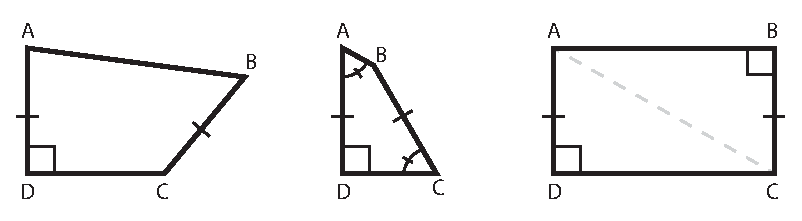
\includegraphics[width=0.95\textwidth]{diagrams/rectangles-answer.eps}
\captionsetup{labelformat=empty}
\caption{{\bf Solution to Example 1:} As the reader likely discovered,
  the first two diagrams can be manipulated to yield instances that
  are not rectangles, while the third is sufficiently constrained to
  always represent a rectangle.  (This can be proven by adding a
  diagonal and using the Pythagorean theorem.)}
\end{figure}

\subsection{Diagrams, Figures, and Constraints}

This example of manipulation using the ``mind's eye'' also introduces
some terminology helpful in discussing the differences between images
as drawn and the spaces of geometric objects they represent.  For
clarity, a \emph{figure} will refer to an actual configuration of
points, lines, and circles drawn on a page.  Constraint annotations
(congruence or measure) placed on objects form a \emph{diagram},
which is the abstract representation of the entire space of figure
\emph{instances} that satisfy the constraints.

An annotated figure presented on a page is typically an instance of
its corresponding diagram.  However, it is certainly possible to add
annotations to a figure that are not satisfied by that figure,
yielding impossible diagrams.  In such a case the diagram represents
an empty set of satisfying figures.

In the initial example above, the three quadrilateral figures are
drawn as rectangles.  It is true that all quadrilateral figures in the
space represented by the third diagram are rectangles.  However, the
space of quadrilaterals represented by the first two diagrams include
instances that are not rectangles, as shown above.  At this time, the
system only works with diagrams whose constraints can be satisfied in
some figure.  Detecting and explaining impossible diagrams, purely
from their set of constraints would be an interesting extension.

\newpage
\section{Geometry Investigation}

These same ``mind's eye'' reasoning techniques can be used to discover
and learn new geometric theorems.  Given some ``interesting
properties'' in a particular figure, one can construct other instances
of the diagram to examine if the properties appear to hold uniformly,
or if they were just coincidences in the initial drawing.  Properties
that are satisfied repeatedly can be further explored and proved using
deductive reasoning.  The examples below provide several
demonstrations of such inductive investigations.

\subsection{Vertical Angles}

\begin{figure}[h!]
\centering
\includegraphics[width=0.95\textwidth]{diagrams/vertical.eps}
\captionsetup{labelformat=empty}
\caption{{\bf Investigation 1:} Construct a pair of vertical angles.
  Notice anything interesting?}
\end{figure}

Often one of the first theorems in a geometry course, the fact that
vertical angles are equal is one of the simplest examples of applying
``mind's eye'' visual reasoning.  Given the diagram on the left, one
could ``wiggle'' the two lines in his or her mind and imagine how the
angles respond.  In doing so, one would notice that the lower angle's
measure increases and decreases proportionately with that of the top
angle.  This mental simulation, perhaps accompanied by a few drawn and
measured figures, could sufficiently convince the viewer that vertical
angles always have equal measure.

Of course, this fact can also be proved deductively by adding up pairs
of angles that sum to 180 degrees, or by using a symmetry arguments.
However, the inductive manipulations are more reflective of the
initial, intuitive process one typically takes when first presented
with understanding a problem.

\newpage
\subsection{Elementary Results}
\label{sec:elem}

\begin{figure}[h!]
\centering
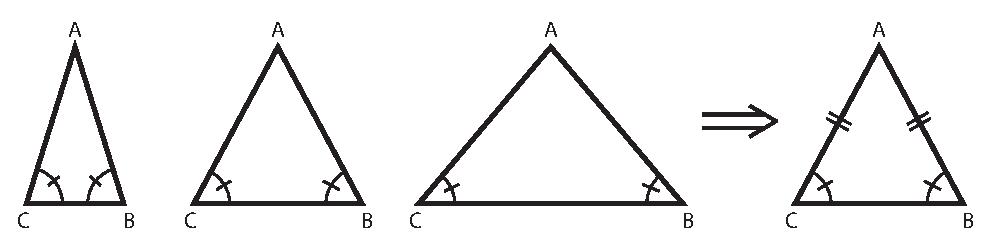
\includegraphics[width=0.95\textwidth]{diagrams/isosceles-triangle.eps}
\captionsetup{labelformat=empty}
\caption{{\bf Investigation 2:} Construct a triangle $ABC$ with
$ \protect\angle B = \protect\angle C$. Notice anything interesting?}
\end{figure}

A slightly more involved example includes discovering that if a
triangle has two congruent angles, it is isosceles.  As above, this
fact has a more rigorous proof that involves dropping an altitude from
point $A$ and using corresponding parts of congruent triangles to
demonstrate the equality of $AB$ and $AC$.  However, the inductive
investigation of figures that satisfy the constraints can yield the
same conjecture, give students better intuition for what is happening,
and help guide the discovery and assembly of known rules to be applied
in future situations.

In this and further examples, an important question becomes what
properties are considered ``interesting'' and worth investigating in
further instances of the diagram, as discussed in Section
\ref{sec:interest}.  As suggested by the examples in Investigation 3,
this can include relations between segment and angle lengths,
concurrent lines, collinear points, or parallel and perpendicular
lines.

\begin{figure}[h!]
\centering
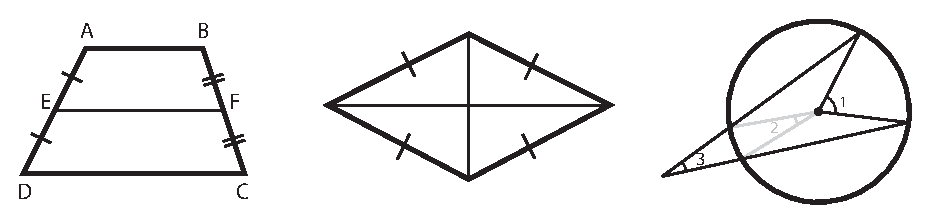
\includegraphics[width=0.95\textwidth]{diagrams/extra-diagrams.eps}
\captionsetup{labelformat=empty}
\caption{{\bf Investigation 3:} What is interesting about the
  relationship between $AB$, $CD$, and $EF$ in the trapezoid? What is
  interesting about the diagonals of a rhombus? What is interesting
  about $\protect\angle 1$, $\protect\angle 2$, and $\protect\angle 3$?}
\end{figure}

\subsection{Nine Point Circle and Euler Segment}

Finally, this technique can be used to explore and discover
conjectures well beyond the scope of what one can visualize in his or
her head:

\begin{figure}[h!]
\centering
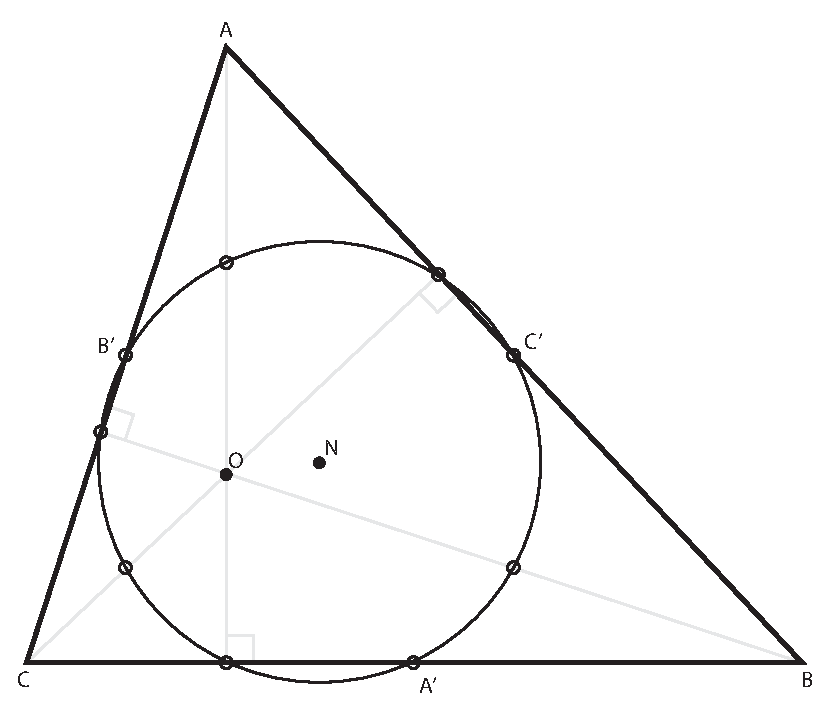
\includegraphics[width=0.8\textwidth]{diagrams/nine-point.eps}
\captionsetup{labelformat=empty}
\caption{{\bf Investigation 4a:} In triangle $ABC$, construct the side
  midpoints $A'$, $B'$, $C'$, and orthocenter $O$ (from altitudes).
  Then, construct the midpoints of the segments connecting the
  orthocenter with each triangle vertex.  Notice anything
  interesting?}
\end{figure}

As a more complicated example, consider the extended investigation of
the Nine Point Circle and Euler Segment.  As shown in Investigation
4a, the nine points created (feet of the altitudes, midpoints of
sides, and midpoints of segments from orthocenter to vertices) are all
concentric, lying on a circle with center labeled $N$.

Upon first constructing this figure, this fact seems almost beyond
chance.  However, as shown in Investigation 4b (next page), further
``interesting properties'' continue to appear as one constructs the
centroid and circumcenter: All four of these special points ($O$, $N$,
$D$, and $M$) are collinear on what is called the \emph{Euler
  Segment}, and the ratios $ON:ND:DM$ of $3:1:2$ hold for any
triangle.

\begin{figure}[h!]
\centering
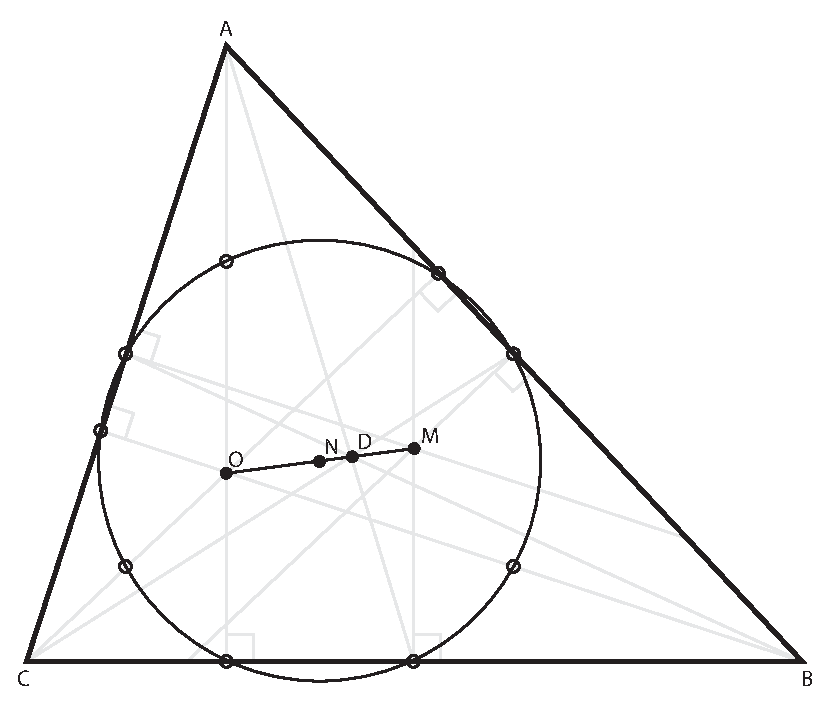
\includegraphics[width=0.8\textwidth]{diagrams/euler-line.eps}
\captionsetup{labelformat=empty}
\caption{{\bf Investigation 4b:} Continue the investigation from 4a by
  also constructing the centroid $D$ (from median concurrence) and
  circumcenter $M$ (from perpendicular bisector concurrence).  Notice
  anything interesting?}
\end{figure}

\section{Discussion}

As the examples and investigations in this chapter demonstrate, mental
manipulation of figures to observe interesting relationships that are
invariant across diagram instances is a useful reasoning skill. Such
relationships can be generalized as conjectures or theorems and used
in further analysis.

The following chapters present an interactive computer system that
emulates this process. Similar to the process of making, manipulating,
and observing pictures ``in the mind's eye'', the system constructs
several examples of figures under investigation and extracts
interesting relationships. A learning module aggregates and applies
the results to new investigations.

\chapter{Demonstration}
\label{chap:demo}

My system uses this idea of manipulating diagrams ``in the mind's
eye'' to explore and discover geometry theorems. Before discussing
some of the internal representations and modules, I will briefly
describe the goals of the system to provide direction and context to
understand the components.

\section{Imperative Figure Construction}

\begin{tcblisting}{colback=white,colframe=black!75!black,
listing only,
leftrule=3pt,
listing options={style=tcblatex,
basicstyle=\footnotesize\ttfamily}}
(define (triangle-with-pep-bisectors)
  (let-geo* ((a (make-point 0 0))
             (b (make-point 1.5 0))
             (c (make-point 1 1))
             (t (polygon-from-points a b c))
             (pb1 (perpendicular-bisector (make-segment a b)))
             (pb2 (perpendicular-bisector (make-segment b c)))
             (pb3 (perpendicular-bisector (make-segment c a))))
    (figure t pb1 pb2 pb3)))
\end{tcblisting}

\begin{tcblisting}{colback=white,colframe=black!75!black,
listing and comment, righthand width=5cm,
leftrule=3pt,
listing options={style=tcblatex,numbers=none,
basicstyle=\footnotesize\ttfamily},
tcbimage comment={images/demo-tri-pb-fig.png},
comment style={size=fbox,colframe=white,colback=white!50,height=8cm},
every listing line*={\textcolor{black}{\small\ttfamily\bfseries => }}}
(show-figure (triangle-with-perp-bisectors))
\end{tcblisting}



\begin{tcblisting}{colback=white,colframe=black!75!black,
listing only, righthand width=5cm,
leftrule=3pt,
fontlower=\ttfamily,
listing options={style=tcblatex,numbers=none,
basicstyle=\footnotesize\ttfamily},
comment style={size=fbox,colframe=white,colback=white!50,height=8cm}}
=> (show-figure (triangle-with-perp-bisectors))

((concurrent #[line 22] #[line 20] #[line 18])
 (perpendicular #[line 22] #[segment 21])
 (perpendicular #[line 20] #[segment 19])
 (perpendicular #[line 18] #[segment 17]))
\end{tcblisting}



\section{Declarative Constraint Solving}

\begin{lstlisting}[caption=Getting labels]
(define (arbitrary-triangle)
  (m:mechanism
   (m:establish-polygon-topology 'a 'b 'c)))
\end{lstlisting}

\begin{lstlisting}[caption=Constraint Solving for Isoceles Triangle]
(define (isoceles-triangle)
  (m:mechanism
   (m:establish-polygon-topology 'a 'b 'c)
   (m:c-length-equal (m:bar 'a 'b)
                     (m:bar 'b 'c))))
\end{lstlisting}


\begin{lstlisting}[caption=Constraint Solving for Isoceles Triangle]
(define (parallelogram-by-angles)
  (m:mechanism
   (m:establish-polygon-topology 'a 'b 'c 'd)
   (m:c-angle-equal (m:joint 'a)
                    (m:joint 'c))
   (m:c-angle-equal (m:joint 'b)
                    (m:joint 'd))))
\end{lstlisting}

\chapter{System Overview}
\label{chap:sys-overview}

This chapter provides an overview of the system. It presents several
concepts relating to input and output representations, introduces the
four main modules, and discusses how they work together in the
discovery of new definitions and theorems.

\section{Goals}

The end goal of the system is for it to notice and learn interesting
concepts in Geometry from inductive explorations. Because these ideas
are derived from inductive observation, I will typically refer to them
as conjectures. Once the conjectures are reported, they can easily be
integrated into existing automated proof systems if a deductive proof
is desired. The conjectures explored can be grouped into three areas:
definitions, properties, and theorems:

\begin{description}

\enlargethispage*{-\baselineskip}

\item[Properties] Properties include all the facts derived from a
  single premise, such as ``Opposite angles in a rhombus are equal''
  or ``The midpoint of a segment divides it into two equal-length
  segments''.

\item[Definitions] Definitions classify and differentiate an object
  from other objects. For instance ``What is a rhombus?'' yields the
  definition that it is a quadrilateral (classification) with four
  equal sides (differentiation). As seen in the demonstration, the
  system will attempt to simplify definition properties to more
  minimal sets, provide alternative formations, and use pre-existing
  definitions when possible: ``A square is a rhombus and a rectangle''

\item[Theorems] Theorems involve relations among additional elements
  constructions from an initial premise. For instance, theorems about
  triangles may involve the construction of angle bisectors, incenters
  or circumcenters, or the interaction among several polygons in the
  same diagram.

\end{description}

Given a repository of these conjectures about geometry, the system
will be able to apply its findings in future investigations by
examining elements to display its knowledge of definitions, and
focusing future investigations by omitting results implied by prior
theorems.

\section{Diagram Representations}

The system and modules are built around three core diagram
representations. As discussed in the motivation section, we use the
term ``diagram'' to represent the abstract geometric object
represented by these means:

\begin{description}

\item[Construction Steps] The main initial representation for most
  diagrams is a series of construction steps. These generally comprise
  the input investigation from an external user trying to teach the
  system a concept. In some investigations, the actual construction
  steps are opaque to the system (as in a teacher that provides a
  process to ``magically'' produce rhombuses), but often, the
  construction steps use processes known by the system so that the
  resulting figures can include dependency information about how the
  figure elements are built.

\item[Analytic Figure] The second representation is an analytic figure
  for a particular instance of a diagram. This representation includes
  coordinates for all points in the diagram and can be displayed. This
  representation is used by the perception module to observe
  interesting relationships.

\item[Symbolic Relationships] Finally, the third representation of a
  diagram is as a collection of symbolic relationships or constraints
  on elements of the diagram. These are initially formed from the
  results of the perception module, but may also be introduced as
  known properties for certain premises and construction steps. These
  symbolic relationships can be further tested and simplified to
  discover which sets of constraints subsume one another.

\end{description}

While construction steps are primarily used as input and to generate
examples, as the system investigates a figure, the analytic figure and
symbolic relationship models get increasingly intertwined. The ``mind's
eye'' perception aspects of observing relationships in the analytic
figure lead to new symbolic relationships and a propagator-like
approach of wigging solutions to the symbolic constraints yields new
analytic figures.

As relationships are verified and simplified, results are output and
stored in the student's repository of geometry knowledge.


\section{Steps in a Typical Interaction}

The system overview figure on the next page depicts the typical
process of interacting with the system and shows relationships between
the four system modules.

These four modules are an imperative geometry construction interpreter
used to build diagrams, a declarative geometry constraint solver to
solve and test specifications, an observation-based perception module
to notice interesting properties, and a learning module to analyze
information from the other modules and integrate it into new
definition and theorem discoveries.

\newpage

\begin{figure}[h!]
\centering
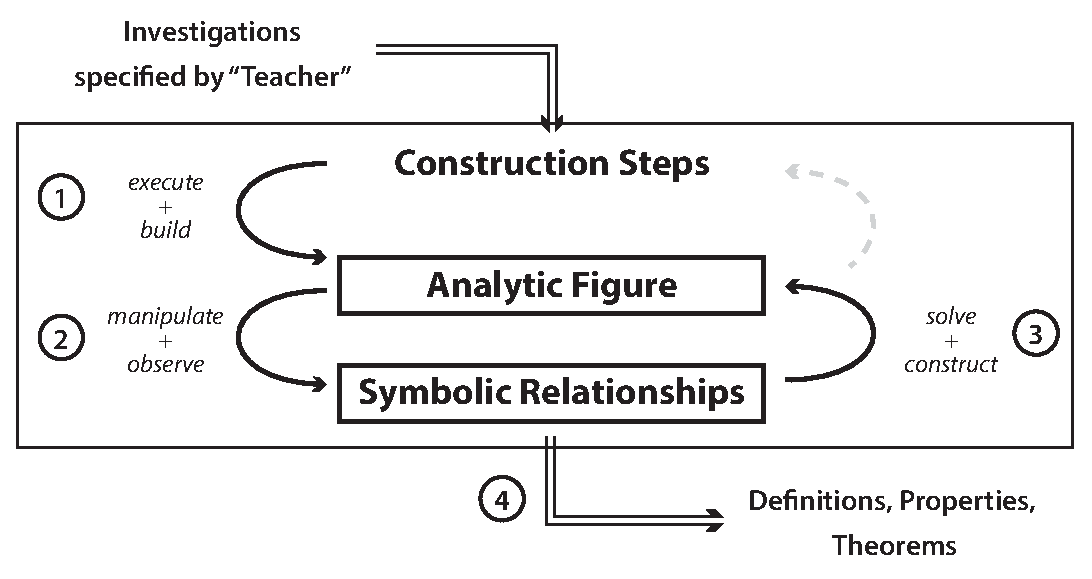
\includegraphics[width=0.9\textwidth]{diagrams/Representations.eps}
\captionsetup{labelformat=empty}
\caption{{\bf System Overview:} Given construction steps for an
  investigation an external teacher wishes the student perform, the
  system first (1) uses its imperative construction module to execute
  these construction steps and build an analytic instance of the
  diagram. Then, (2) it will manipulate the diagram by ``wiggling''
  random choices and use the perception module to observe interesting
  relationships. Given these relationships, it will (3) use the
  declarative propagator-based constraint solver to reconstruct a
  figure satisfying a subset of the constraints to determine which are
  essential in the original diagram. Finally (4), a learning module
  will monitor the overall process, omit already-known results, and
  assemble a repository of known definitions, properties, and
  theorems.}
\end{figure}

\subsection{Interpreting Construction Instructions}

\enlargethispage*{\baselineskip}

The first step in an exploration is interpreting an input of the
diagram to be investigated.  The imperative construction module takes
as input explicit construction steps that results in an instance of
the desired diagram.  These instructions can still include arbitrary
selections (let $P$ be some point on the line, or let $A$ be some
acute angle), but otherwise are restricted to basic construction
operations that could be performed using a compass and straight edge.

To simplify the input of more complicated diagrams, some of these
steps can be abstracted into a library of known construction
procedures.  For example, although the underlying figures are limited
to very simple objects of points, lines, and angles, the steps of
constructing a triangle (three points and three segments) or bisecting
a line or angle are encapsulated into single steps.

\subsection{Creating Figures}

Given a language for expressing the constructions, the second phase of
the system is to perform such constructions to yield an instance of
the diagram.  This process mimics ``imagining'' images and results in
an analytic representation of the figure with coordinates for each
point.  Arbitrary choices in the construction (``Let $Q$ be some point
on the line.'') are chosen via an random process, but with an attempt
to keep the figures within a reasonable scale to ease human
inspection.

\subsection{Noticing Interesting Properties}
\label{sec:interest}

Having constructed a particular figure, the system examines it to find
interesting properties.  These properties involve facts that appear to
be ``beyond coincidence''.  This generally involves relationships
between measured values, but can also include ``unexpected''
configurations of points, lines, and circles.  As the system discovers
interesting properties, it will reconstruct the diagram using
different choices and observe if the observed properties hold true
across many instances of a diagram.

\subsection{Reporting and Simplifying Findings}

Finally, once the system has discovered some interesting properties
that appear repeatedly in instances of a given diagram, it reports its
results to the user via the learning module.  Although this initially
includes a simple list of all simple relationships, effort is taken to
avoid repeating observations that obvious in the construction.  For
example, if a perpendicular bisector of segment $AB$ is requested, the
fact that it bisects that segment in every instance is not
informative.  To do so, the construction process interacts with
properties known in the learning module to maintain a list of facts
that can be reasoned from construction assumptions so that these can
be omitted in the final reporting. Finally, given several properties
true of a figure, the learning module uses the constraint solver in an
attempt to reconstruct a figure satisfying a subset of the constraints
to determine which are essential in the original diagram.

\chapter{Imperative Construction System}
\label{chap:imperative}

\section{Overview}

The first module is an imperative system for performing geometry
constructions. This is the typical input method for generating
coordinate-backed instances of figures and thus declares.

We will first discuss the basic underlying structures that comprise
figures, then describe the higher-order language used to specify
construction steps.

\section{Basic Structures}

\subsection{Points}

Points form the basis of most elements. Throughout the system, points
are labeled and used to identify other elements.

\section{Linear Elements}

The linear elements of Segments, Lines, and Rays are built upon
points. Initially the internal representation of lines were that of
two points, but to simplify manipulations,

To better specify angles (see below), all linear elements, including
segments and lines are directioned. Thus, a line pointing. Predicates
exist that compare lines for equality ignoring

\subsection{Angles}

Initially angles were represented as three points, now vertex + two
directions. CCW orientation. Methods exist to determine them from
various pairs of linear elements, uses directionality of linear
elements to determine which ``quadrant'' of the angle is desired.

Given a figure, methods exist to extract angles from the diagrams in
analysis rather than specifying each angle of interest while creating
the diagram.

\subsection{Math Support}

Some ``core'' math structures to help these calculations: Direction
represents a direction in [0, 2pi], fixes principal value [0, 2pi],
and support various operations for direction intervals (basic
intersection, adding, shifting, etc). Currently all represented by
single theta value, could generalize via generics to dx, dy, or theta
depending on computation source.

\section{Higher-level structures}

In addition to the basic geometry structures, the system uses several
grouping structures to combine and abstract the basic figure elements
into higher-level figures elements.

For closure of combinators, all these higher level objects are also
``Diagram objects''.

\subsection{Polygons}

Polygons are represented as groups of points.

\subsection{Figures}

Figures are currently groups of elements. In the creation of figures
we extract additional information and build a graph out of adjacent
components for use in the analysis stages.

\section{Construction Operations}

\subsection{Traditional constructions}

Midpoint, perpendicular line, bisectors

\subsection{Intersections}

Generic intersections, mathematically based at line/line or
line/circle at the core. Other intersections also add the check that
the resulting point(s) are on the elements.

\subsection{Measurement-based operations}

A ``Ruler + Protractor'' is generally not permitted in traditional
construction problems. However, sometimes its nice to be able to use
measurements to more quickly compute a result (e.g.\ angle bisector by
halving angle) vs.\ going through the whole ray/circle based
construction process.

\subsection{Transformations}

Currently, rotate about a point or translate by a vector. Also
interfaces for by *random* point or vector.

\section{Randomness}

\subsection{Random Choices}

At the basis of all random

\subsection{Remembering choices}

\subsection{Backtracking}

Currently, the system does not backtrack based on random
choices. However, there are plans to perform checks on
randomly-generated elements that are too close to one another and to
retry the random choice to avoid degenerate choices.

\subsection{Avoiding almost-degenerate points}

As discussed above, randomly making choices in

\subsection{Animating choices}

I animate over a small range within the specified random
range. Top-level infrastructure determinies frames, sleeping, etc.
Constructions can request to animate functions of one arg [0, 1]. As
the figure and animation is run, each call to randomize gets a call to
random whenever their value is non-false.

\section{Dependencies}

\subsection{Implementation}

Eq-properties, etc.

\subsection{Naming}

Sometimes derived if unknown, figure out how name metadata relates to
the dependencies.

\subsection{Forcing higher-level random dependenceis}

"Inverts" the dependency tree that would otherwise usually go
down to points. set-dependency! as random-square. When given an
element by the teacher, generally we don't know how the construction
was performed.

\subsection{Dependency-less diagrams}

In some cases, the dependency structure of a figure can be wiped.

\section{Construction Language}

Constructions and instruction-based investigations are specified by
scheme procedures that return the desired figures.

\subsection{Macros}

I created a let-geo* special form that is similar to Scheme's (let
...) form, but sets the element names as specified so they can be more
easily referred to later.

\subsection{Multiple Assignment}

In let-geo*, I also permit some constructions to optionally map to
multiple assignments of names, such as the case in which you create a
triangle and simulatneously want to store and name the triangle's
vertex points.

\section{Graphics}

The system integrates with Scheme's graphics system for the X Window
System to display the figures for the users. The graphical viewer can
include labels and highlight specific elements, as well as display
animations representing the ``wiggling'' of the diagram.

\chapter{Perception Module}
\label{chap:observer}

%% Outline
%% - Relationships
%% - Observations
%% - Full Analysis Procedure
%% - Auxillary Segments
%% - Discussion

\section{Overview}

The perception module focuses on ``seeing'' figures in our mind's eye.
Given analytic figures represented using structures of the imperative
construction module, the perception module is concerned with finding
and reporting interesting relationships seen in the figure. In a
generate-and-test-like fashion, it is rather liberal in the
observations it returns. The module uses several technique to attempt
to omit obvious properties, and combines with the learning module
(Chapter~\ref{chap:learning}) to filter already-learned discoveries
and simplify results.

To explain the module, I will first describe the implementation of
underlying relationship and observation structures before examining
the full analyzer routine. I will conclude with a discussion of
extensions to the module, including further ways to detect and remove
obvious results and some attempted techniques used to extract
auxiliary relationships from figures.

\section{Relationships}

Relationships are the primary structures defining what constitutes
interesting properties in a figure. Relationships are represented as
predicates over typed n-tuples and are checked against all such
n-tuples found in the figure under analysis.

\begin{code-listing}
[label=relationship-structure]
{Relationships}
(define-record-type <relationship>
  (make-relationship type arity predicate equivalence-predicate)
  relationship?
  (type relationship-type)
  (arity relationship-arity)
  (predicate relationship-predicate)
  (equivalence-predicate relationship-equivalence-predicate))

(define equal-length-relationship
  (%make-relationship 'equal-length 2 segment-equal-length?
                      (set-equivalent-procedure segment-equivalent?)))

(define concurrent-relationship
  (make-relationship 'concurrent 3 concurrent?
                      (set-equivalent-procedure linear-element-equivalent?)))

(define concentric-relationship
  (make-relationship 'concentric 4 concentric?
                      (set-equivalent-procedure point-equal?)))
\end{code-listing}

Listing~\ref{relationship-structure} displays some representative
relationships.  The relationship predicates can be arbitrary Scheme
procedures and often use constructions and utilities from the
underlying imperative system as seen in
Listing~\ref{concurrent-concentric}.  \texttt{concurrent?} is checked
over all 3-tuples of linear elements (lines, rays, segments) and
\texttt{concentric?} is checked against all 4-tuples of points.

\begin{code-listing}
[label=concurrent-concentric]
{Concurrent and Concentric Predicates}
(define (concurrent? l1 l2 l3)
  (let ((i-point (intersect-linear-elements-no-endpoints l1 l2)))
    (and i-point
         (on-element? i-point l3)
         (not (element-endpoint? i-point l3)))))

(define (concentric? p1 p2 p3 p4)
  (and (distinct? p1 p2 p3 p4)
       (let ((pb-1 (perpendicular-bisector (make-segment p1 p2)))
             (pb-2 (perpendicular-bisector (make-segment p2 p3)))
             (pb-3 (perpendicular-bisector (make-segment p3 p4))))
         (concurrent? pb-1 pb-2 pb-3))))
\end{code-listing}

In addition to the type, arity, and predicate checked against
arguments, the relationship structures also include an equivalence
predicate that is used in determining whether two observations using
the relationship are equivalent, as will be discussed after
explaining the observation structure in Section~\ref{sec:obs}.

\subsection{What is Interesting?}
The system currently checks for:
\begin{spacing}{0.7}
\begin{itemize}
\item concurrent, parallel, and perpendicular linear elements,
\item segments of equal length,
\item supplementary and complementary angles,
\item angles of equal measure,
\item coincident and concentric points, and
\item sets of three concentric points with a fourth as its center.
\end{itemize}
\end{spacing}
\noindent These relationships covered most of the basic observations needed in
my investigations, but further relationships can be easily added.

\section{Observations}
\label{sec:obs}

Observations are structures used to report the analyzer's findings. As
seen in Listing~\ref{obs}, they combine the relevant relationship
structure with a list of the actual element arguments from the figure
that satisfy that relationship. Maintaining references to the actual
figure elements allows helper procedures to print names or extract
dependencies as needed.

\begin{code-listing}
[label=obs]
{Observations}
(define-record-type <observation>
  (make-observation relationship args)
  observation?
  (relationship observation-relationship)
  (args observation-args))
\end{code-listing}

It is important to know whether two arbitrary observations are
equivalent. This enables the system to detect and avoid reporting
redundant or uninteresting relationships.  Listing~\ref{eqv-obs} shows
the implementation of \texttt{observation-equivalent?}. The procedure
checks the observations are the same and then applies that
observation's equivalence predicate to the two tuples of observation
arguments.

\begin{code-listing}
[label=eqv-obs]
{Equivalent Observations}
(define (observation-equivalent? obs1 obs2)
  (and (relationship-equal?
        (observation-relationship obs1)
        (observation-relationship obs2))
       (let ((rel-eqv-test
              (relationship-equivalence-predicate
               (observation-relationship obs1)))
             (args1 (observation-args obs1))
             (args2 (observation-args obs2)))
         (rel-eqv-test args1 args2))))
\end{code-listing}

These equivalence predicates handle the various patterns in which
objects may appear in observations. For example, in an observation
that two segments have equal length, it does not matter which segment
comes first or which order the endpoints are listed within each
segment. Thus, as shown in Listing~\ref{segment-equal-eqv}, the
equivalence procedure ignores these ordering differences by comparing
set equalities:

\begin{code-listing}
[label=segment-equal-eqv]
{Equivalence of Equal Segment Length Observations}
(set-equivalent-procedure segment-equivalent?)

(define (set-equivalent-procedure equality-predicate)
  (lambda (set1 set2)
    (set-equivalent? set1 set2 equality-predicate)))

(define (set-equivalent? set1 set2 equality-predicate)
  (and (subset? set1 set2 equality-predicate)
       (subset? set2 set1 equality-predicate)))

(define (segment-equivalent? s1 s2)
  (set-equivalent?
   (segment-endpoints s1)
   (segment-endpoints s2)
   point-equal?))

(define (point-equal? p1 p2)
  (and (close-enuf? (point-x p1) (point-x p2))
       (close-enuf? (point-y p1) (point-y p2))))
\end{code-listing}

\subsection{Numerical Accuracy}

Throughout the system, numerical accuracy issues and floating point
errors arise when comparing objects. As a result, the system uses
custom equality operators for each data type, such as
\texttt{point-equal?} shown in Listing~\ref{segment-equal-eqv}. These
use an underlying floating-point predicate \texttt{close-enuf?} taken
from the MIT Scheme Mathematics Library \cite{scmutils} that estimates
and sets a tolerance based on current machine's precision and handles
small magnitude values intelligently. With this floating point
tolerance in comparisons, floating point errors have been
significantly less prevalent.

\section{Analysis Procedure}

Given these relationship and observation structures,
Listing~\ref{analyzer} presents the main analyzer routine in this
module. After extracting various types of elements from the figure, it
examines the relationships relevant for each set of elements and
gathers all resulting observations.

\begin{code-listing}
[label=analyzer]
{Analyzer Routine}
(define (analyze figure)
  (let* ((points (figure-points figure))
         (angles (figure-angles figure))
         (linear-elements (figure-linear-elements figure))
         (segments (figure-segments figure)))
    (append
     (extract-relationships points
                            (list concurrent-points-relationship
                                  concentric-relationship
                                  concentric-with-center-relationship))
     (extract-relationships segments
                             (list equal-length-relationship))
     (extract-relationships angles
                             (list equal-angle-relationship
                                   supplementary-angles-relationship
                                   complementary-angles-relationship))
     (extract-relationships linear-elements
                             (list parallel-relationship
                                   concurrent-relationship
                                   perpendicular-relationship)))))
\end{code-listing}

The workhorses of \texttt{extract-relationships} and
\texttt{report-n-wise} shown in Listing~\ref{extract-relationships}
generate the relevant n-tuples and report observations for those that
satisfy the relationship under consideration. For these homogeneous
cases, \texttt{all-n-tuples} returns all (unordered) subsets of size
$n$ as lists.

\begin{code-listing}
[label=extract-relationships]
{Extracting Relationships}
(define (extract-relationship elements relationship)
  (map (lambda (tuple)
         (make-observation relationship tuple))
       (report-n-wise
        (relationship-arity relationship)
        (relationship-predicate relationship)
        elements)))

(define (report-n-wise n predicate elements)
  (let ((tuples (all-n-tuples n elements)))
    (filter (nary-predicate n predicate) tuples)))
\end{code-listing}

\section{Focusing on Interesting Observations}

The final aspect of the perception module involves filtering out
obvious and previously-discovered observations.  Several techniques
will be discussed but Listing~\ref{interesting-obs-impl} shows the
module's current state of accomplishing this task via the
\texttt{interesting-observations} procedure. The procedure first
extracts all observations from the figure and aggregates a list of
obvious relations specified during the construction. It then uses the
learning module to examine all polygons found in the figure and
determine the most specific definitions each satisfies. The procedure
obtains in \texttt{polygon-implied-observations} all
previously-discovered facts about such shapes to remove from the final
result and adds new polygon observations in their
place. Example~\ref{cyc-interesting} shows a concrete example of this.

\newpage

\begin{code-listing}
[label=interesting-obs-impl]
{Obtaining Interesting Observations}
(define (interesting-observations figure-proc)
  (set! *obvious-observations* '())
  (let* ((fig (figure-proc))
         (all-obs (analyze-figure fig))
         (polygons (figure-polygons fig))
         (polygon-observations (polygon-observations polygons))
         (polygon-implied-observations
           (polygon-implied-observations polygons))
    (set-difference (append all-obs polygon-observations)
                    (append *obvious-observations* polygon-implied-observations)
                    observation-equivalent?)))
\end{code-listing}

Listing~\ref{mark-obvious} shows the implementation of the
\texttt{save-obvious-observation!} procedure

\begin{code-listing}
[label=mark-obvious]
{Marking Obvious Observations}
(define (save-obvious-observation! obs)
  (if *obvious-observations*
      (set! *obvious-observations*
            (cons obs *obvious-observations*))))
\end{code-listing}

Example~\ref{interesting-analysis} in the demonstration chapter
demonstrated a simple example of a construction procedure that marked
obvious properties of its results.

\begin{img-example}
[label=cyc-interesting]
{Substituting Polygon Observations}
{images/inner-investigation-1.png}
Observations
\end{img-example}

\section{Discussion and Extensions}

Perfectly determining is a large task, particularly since filtering
out obvious relations often requires relationship-specific information:

As one example, imagine implementing and a \texttt{collinear?}
predicate that only reports non-obvious relations. Testing whether
three arbitrary coordinate-based points are collinear is
straightforward. However, it is not interesting that a random point on
a line is collinear with the two points from which the line was
defined. In order to accurately know whether or not it is interesting
that three points are collinear, the system would need to have access
to a graph-like representation of which points were specified to be on
which lines.

The analysis routine was initially one large, arbitrarily complicated
procedure in which individual checks were added. This reformulation to
use relationships and observations has simplified the complexity and
enabled better interactions with the learning module, but limited the
ability for adding many relationship-specific optimizations.

Despite these limitations, the perception system has been sufficient
to discover several relations via the learning model and use basic
filtering of obvious relations to present intelligible results.

The examples below describe further efforts explored for improving the
perception module. This involves extracting relationships for elements
not explicitly specified in a figure, such as auxiliary segments
between all pairs of points in the figure, treating all intersections
as points, extracting angles, or merging results. These are areas for
future work.

\subsection{Auxiliary Segments}

In some circumstances, the system can insert and consider segments
between all pairs of points. Although this can sometimes produce
interesting results, it can often lead to too many elements being
considered. This option is off by default but could be extended and
enabled in a self-exploration mode.

\subsection{Extracting Angles}

In addition, I briefly explored a system in which the construction
module also maintains a graph-like representation of the connectedness
and adjacencies in the figure. In addition to the complexity of
determining which angles to keep, keeping track of ``obvious''
relationships between such extracted angles due to parallel lines, for
instance, is quite a challenge.

\subsection{Merging Related Observations}

A final process I explored involved merging related observations into
larger, combined results. For instance, when reporting segment length
equality for a square, it is excessive to report all possible pairs of
equal sides.

%% Initial Stuff:

\if false

\subsection{Extracting segments and angles}

The observation module also builds and traverses a
graph-representation of the object of connectedness and adjacencies to
extract more segments and angles, or include intersections of elements
in its investigation.

\subsection{Removing Obvious Properties}

This module makes use of available dependency information to eliminate
some obvious properties. At this phase, the eliminations arise only
from basic geometry knowledge ``hard-coded'' into the system, and not
upon any specific prior-learned formula.

\subsubsection{Trivial relations}

Points being on lines, segments, circles directly dependent on that point.

\subsubsection{Branch Relations}

Other examples include ``branch'' relations. [REF: Chen, Song,
  etc.]. ABCD on a line with AB = CD also means that AC = BD, for instance.

\section{Representations}

A ``Relationship'' object represents a type of relationship, a
``Observation'' object refers to a specific observation seen in a
figure.

\fi

\chapter{Declarative Geometry Constraint Solver}
\label{chap:declarative}

\section{Overview}

The third module is a declarative geometry constraint solver. Given a
user-specified topology of a diagram and various constraints on
segments and angles, this module attempts to solve the specification
by instantiating a figure that satisfies the constraints.

The solver is implemented using propagators, uses new types of partial
information about point regions and direction intervals, and focuses
on emulating the mental process of wiggling constrained figures in the
mind's eye. The physical nature of this process is captured by forming
analogies between geometry diagrams and mechanical linkages of bars
and joints.

After providing a brief overview of the mechanical analogies and quick
background on the propagator system, I examine an example of the
system solving a set of constraints for an under-constrained
rectangle. Then, I describe the module implementation, starting with
the new partial information representations and linkage constraints
before explaining how mechanisms are assembled and solved. Finally,
some limitations and extensions are discussed.

%% Outline
%% - Mechanical Analogies
%% - Propagator System
%% - Partial Information Structures
%% - Linkages
%% - Building a Mechanism
%% - Solving a Mechanism
%% - Discussion

\section{Mechanical Analogies}

Mechanical analogies are often applied to mathematical problems to
yield alternate, sometimes more-intuitive solutions. Several texts
such as [??], [??], and [??] study this and provide examples.

In this system, mechanical analogies are used to represent the physics
simulation going on as one mentally manipulates a diagram ``in the
mind's eye''. Often, given a diagram with constraints, one can imagine
assembling a physical example of the figure out of bars and joints in
one's head.  Some bars can be sliding to make their lengths adjustable
whereas others are constrained to be of equal length as one another.
As a person moves and wiggles these pieces to assemble satisfying
mechanisms, they can examine whether the resulting mechanisms retain
properties across instances and generalize such invariants into
theorems.

This module simulates this process by assembling mechanisms of bars
and joints, and using a propagator system to simulate incrementally
selecting where bars and joints are positioned while maintaining local
physical constraints.

\section{Propagator System}

The declarative geometry solver is built upon an existing propagator
system created by Alexey Radul under the advisement of Gerald Jay
Sussman \cite{gjs-propagator}. The propagator system allows a user to
create cells and connect them with propagator constraints. As content
is added to cells, their neighbors are notified and updated with
computations performed on the new information. Often, cells maintain a
representation of partial information about their content and merge
new information from several sources.

This module uses Radul's propagation system to handle the underlying
propagation of data, but implements constraints, partial information
types, specification protocols, and input formats particular to geometric
figures.

\section{Example of Solving Geometric Constraints}
\label{sec:example-solving}

I begin by fully explaining an example. The geometry problem of
inadequately constrained rectangles was introduced in the first
example of Chapter~\ref{chap:motivation} on page
\pageref{example-1}. The second proposed set of constraints in that
problem was expressed as a mechanism in Example~\ref{is-rect-2} in the
demonstration (page \pageref{is-rect-2}), and is repeated here in
Example~\ref{is-rect-specs}. Example~\ref{is-rect-solved} shows the
module's print messages as it solves the mechanism.

The illustrations in Explanation~\ref{illustration} and accompanying text
on the following pages explain how propagation is used to solve this
mechanism.

\begin{code-example}
[label=is-rect-specs]
{Rectangle Constraints Example}
(define (is-this-a-rectangle-2)
  (m:mechanism
   (m:establish-polygon-topology 'a 'b 'c 'd)
   (m:c-length-equal (m:bar 'a 'd) (m:bar 'b 'c))
   (m:c-right-angle (m:joint 'd))
   (m:c-angle-equal (m:joint 'a) (m:joint 'c))))
\end{code-example}

\begin{img-example}
[label=is-rect-solved]
{Solved Constraints}{images/rect-demo-2.png}
=> (m:run-mechanism (is-this-a-rectangle-2))

(specifying-bar m:bar:d:a .6742252545577186)
(initializing-direction m:bar:d:a-dir (direction 4.382829365403101))
(initializing-point m:bar:d:a-p1 (0 0))
(specifying-joint m:joint:c:b:a 2.65583669872538)
\end{img-example}

Solving a mechanism involves repeatedly selecting positions, lengths,
angles, and directions that are not fully specified and selecting
values within the domain of that element's current partial
information. As values are specified, the wiring of the propagator
model propagates further partial information to other values.

\refstepcounter{tcb@cnt@code-example}\label{illustration}
\begin{figure}[h]
\captionsetup{labelformat=empty}
\caption{{\bf Propagation Explanation
    \arabic{chapter}.\arabic{tcb@cnt@code-example}:} This series of
  illustrations depicts the propagation steps that occur to enable the
  system to solve the underconstrained rectangle from
  Example~\ref{is-rect-specs}.
}
\centering
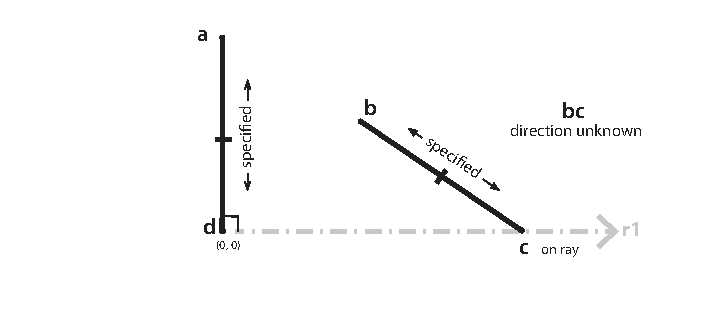
\includegraphics[width=.95\textwidth]{diagrams/is-rect-explained-boards-1.eps}
\caption{{\bf Step 1:} The first value the module specifies is the
  length of bar \texttt{ad}. In doing so, it also initializes the
  bar's endpoint and direction to anchor it on the canvas. Because
  joint \texttt{d} is constrained to be a right angle, the system knows
  the direction but not length of bar \texttt{dc}. It propagates the
  partial information that point \texttt{c} is on the ray $r1$ extending
  out from \texttt{d} to the cell within point
  \texttt{c}. Furthermore, since bars \texttt{ad} and \texttt{bc} are
  constrained to have equal length, at this point, bar \texttt{bc} also knows
  its length but not direction. Next, the system specifies joint angle \texttt{b}:}
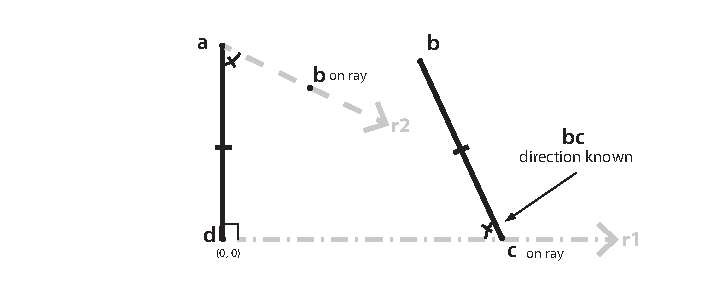
\includegraphics[width=.95\textwidth]{diagrams/is-rect-explained-boards-2.eps}
\caption{{\bf Step 2:} Once the angle measure of \texttt{b} is
  specified, constraints using the sum of angles in the specified
  polygon and a ``slice'' constraint on the pair of constrained angles
  will set the angle measures of joints \texttt{a} and \texttt{c} to
  be half of the remaining total:
  $\text{\texttt{a,c}}\protect\leftarrow\frac{2\protect\pi -
    \text{\texttt{b}} - \text{\texttt{d}}}{2}$. With these angles
  specified, point \texttt{b} is informed that it is on the ray $r2$
  and bar \texttt{bc} now knows both its length and direction.}
\vspace{-10em}
\end{figure}

\newpage
\begin{figure}[h]
\captionsetup{labelformat=empty}
\caption{{\bf Propagation Explanation
    \arabic{chapter}.\arabic{tcb@cnt@code-example} continued:} This series of
  illustrations depicts the propagation steps that occur to enable the
  system to solve the underconstrained rectangle solved in
  Example~\ref{is-rect-specs}.}
\centering
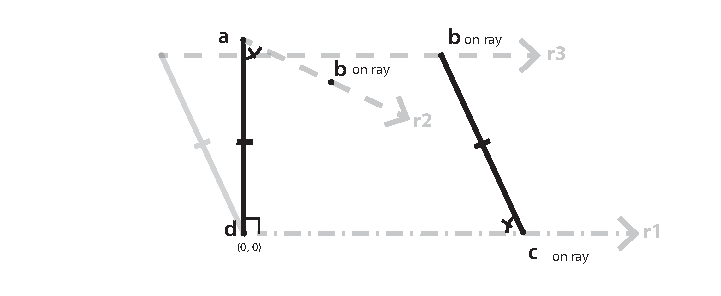
\includegraphics[width=.95\textwidth]{diagrams/is-rect-explained-boards-3.eps}
\caption{{\bf Step 3:} Since now both the length and direction of bar
  \texttt{bc} are known and point \texttt{c} is known to be on ray
  $r1$, the propagation constraints can translate this ray by the
  length and direction of \texttt{bc} and provide the information that
  point \texttt{b} must therefore also be on ray $r3$. This emulates
  the physical process of sliding bar \texttt{bc} along ray $r1$.}
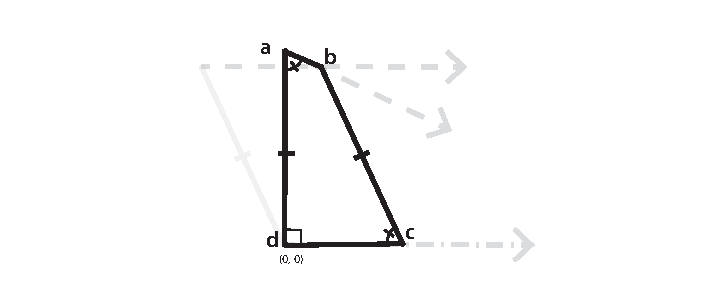
\includegraphics[width=.95\textwidth]{diagrams/is-rect-explained-boards-4.eps}
\caption{{\bf Step 4:} The information about point \texttt{b} being on
  rays $r2$ and $r3$ is merged via ray intersection to fully determine
  the location of \texttt{b}. Then, once point \texttt{b} is
  specified, since the length and direction of bar \texttt{bc} is
  known, propagation sets the value and location of point \texttt{c},
  yielding a fully-specified solution.}
\vspace{-1.5em}
\end{figure}
Similar steps allow propagation to solve specifications for many
figures including isoceles triangles, parallelograms, and
quadrilaterals from their diagonals. Several of these are shown in
Section \ref{demo:sec:declarative}. In cases when bars have their
length and one endpoint specified first, the propagators specify that
the other endpoint is on an arc of a circle. The next sections
describe the implementation of these partial information structures
before explaining linkages and how mechanisms are built and solved.

\newpage
\section{Partial Information Structures}

\subsection{Regions}

Propagating partial information across bars and joints yields a new
region system: Regions include point sets of one or more possible
points, an entire ray, or an entire arc. These rays and arcs are
from an anchored bar with only one of direction or length specified,
for instance.

\subsection{Direction Intervals}

Ranges of intervals. Full circle + invalid intervals. Adding and
subtracting intervals of direction and thetas gets complicated at times.

Challenges with intersection, multiple segments. Eventually just
return nothing is okay.

\section{Bar and Joint Linkages}

Bars have endpoints, directions and length. Joints have a vertex point
and two directions. Currently, most joints are directioned and have
max value of 180 degrees.

\section{Propagator Constraints}

System uses propagators to solve these mechanism constraints.

\subsection{Basic Linkage Constraints}

Direction, dx, dy, length, thetas. ``Bars'' + ``Joints''

\begin{code-listing}{Basic Bar Constraints}
(define (m:make-bar bar-id)
  (let ((bar-key (m:make-bar-name-key bar-id)))
    (let ((p1 (m:make-point (symbol bar-key '-p1)))
          (p2 (m:make-point (symbol bar-key '-p2))))
      (name! p1 (symbol bar-key '-p1))
      (name! p2 (symbol bar-key '-p2))
      (let ((v (m:make-vec bar-key)))
        (c:+ (m:point-x p1)
             (m:vec-dx v)
             (m:point-x p2))
        (c:+ (m:point-y p1)
             (m:vec-dy v)
             (m:point-y p2))
        (let ((bar (%m:make-bar p1 p2 v)))
          (m:p1->p2-bar-propagator p1 p2 bar)
          (m:p2->p1-bar-propagator p2 p1 bar)
          bar)))))
\end{code-listing}

\subsection{User-specified Constraints}

\begin{code-listing}{User Constraints}
(define-record-type <m:constraint>
  (m:make-constraint type args constraint-procedure)
  m:constraint?
  (type m:constraint-type)
  (args m:constraint-args)
  (constraint-procedure m:constraint-procedure))

(define (m:c-length-equal bar-id-1 bar-id-2)
  (m:make-constraint
   'm:c-length-equal
   (list bar-id-1 bar-id-2)
   (lambda (m)
     (let ((bar-1 (m:lookup m bar-id-1))
           (bar-2 (m:lookup m bar-id-2)))
       (c:id
        (m:bar-length bar-1)
        (m:bar-length bar-2))))))
\end{code-listing}

Angle sum of polygon, or scan through polygon and ensure that the
angles don't not match. Example is equilateral triangle, for
instance... Could also observe always ``60 degrees'' as an interesting
fact and put that in as a constraint. They're alebgraically quite
similar, but my propagators currently don't perform symbolic algebra.

\subsection{Building Mechanisms}

The Mechanism in our declarative system is analogous to Figure,
grouping elements. Also computes various caching and lookup tables to
more easily access elements.

\begin{code-listing}
[label=est-topo]
{Establishing Topology}
(define (m:establish-polygon-topology . point-names)
  (if (< (length point-names) 3)
      (error "Min polygon size: 3"))
  (let ((extended-point-names
         (append point-names
                 (list (car point-names) (cadr point-names)))))
    (let ((bars
           (map (lambda (p1-name p2-name)
                  (m:make-named-bar p1-name p2-name))
                point-names
                (cdr extended-point-names)))
          (joints
           (map (lambda (p1-name vertex-name p2-name)
                  (m:make-named-joint p1-name vertex-name p2-name))
                (cddr extended-point-names)
                (cdr extended-point-names)
                point-names)))
      (append bars joints
              (list (m:polygon-sum-slice
                     (map m:joint-name joints)))))))
\end{code-listing}

\begin{code-listing}
{Building Mechanisms}
(define (m:build-mechanism m)
  (m:identify-vertices m)
  (m:assemble-linkages (m:mechanism-bars m)
                       (m:mechanism-joints m))
  (m:apply-mechanism-constraints m)
  (m:apply-slices m))
\end{code-listing}

\section{Solving Mechanisms}

\begin{code-listing}
[label=solve-mechanism]
{Solving Mechanisms}
(define (m:solve-mechanism m)
  (m:initialize-solve)
  (let lp ()
    (run)
    (cond ((m:mechanism-contradictory? m)
           (m:draw-mechanism m c)
           #f)
          ((not (m:mechanism-fully-specified? m))
           (if (m:specify-something m)
               (lp)
               (error "Couldn't find anything to specify.")))
          (else 'mechanism-built))))
\end{code-listing}

Given a wired diagram, process is repeatedly specifying values for elements


\subsection{Interfacing with existing diagrams}

Converts between figures and symbolic relationships.

\section{Discussion and Extensions}

Future efforts involve an improved backtrack-search mechanism if
constraints fail, and a system of initializing the diagram with
content from an existing figure, kicking out and wiggling arbitrary
premises, and seeing how the resulting diagram properties respond.

\subsection{Backtracking}

If it can't build a figure with a given set of specifications, it will
first try some neighboring values, then backtrack and try a new value
for the previous element. After a number of failed attempts, it will
abort and claim that at this time, it is unable to build a diagram
satisfying the constraints.

\chapter{Learning Module}
\label{chap:learning}

\section{Overview}

As the final module, the learning module integrates information from
the other modules and provides the primary, top-level interface for
interacting with the system. It provides means for users to query its
knowledge and provide investigations for the system to carry
out. Through performing such investigations, the learning module
formulates conjectures based on its observations and maintains a
repository of information representing a student's understanding of
geometry concepts.

I will first discuss the interface for interacting with the
system. Then, after describing the structures for representing and
storing definitions and conjectures, I demonstrate how the system
module new terms and conjectures. Finally, I will explain the cyclic
interaction between the imperative and declarative modules used to
simplify definitions and discuss some limitations and future
extensions.

The Demonstration Chapter (Sections~\ref{sec:end-goal-1}
and~\ref{sec:end-goal-2}) included several use cases and examples of
working with the learning module. As a result, this discussion will
focus on structures and implementation rather than uses and
applications. Refer to the demonstration for examples.

%% Outline
%% - Interface (what-is, etc.) / Student
%% - Definitions and Conjectures, Lattice
%% - Learning terms and conjectures
%% - Simplifying definitions
%% - Discussion

\section{Learning Module Interface}

As seen in the demonstration, the learning module provides the primary
interface by which users interact with the system. As such, it
provides means by which users can both query the system to discover
and use what it has known, as well as to teach the system information
by suggesting investigations it should
undertake. Listing~\ref{l-interface} shows the implementation for some
of these methods.

\begin{code-example}
[label=l-interface]
{Learning System Interface Examples}
(define (what-is term)
  (pprint (lookup term)))

(define (example-object term)
  ((definition-generator (lookup term))))

(define (show-example term)
    (show-element (example-object term))

(define (is-a? term obj)
  (let ((def (lookup term)))
    (definition-holds? def obj)))

(define (examine object)
  (let ((satisfying-terms
         (filter (lambda (term) (is-a? term object))
           (known-terms))))
    (remove-supplants more-specific? satisfying-terms)))
\end{code-example}

Explaining these interface implementations provide a context for
introducing the representation of definitions and conjectures.
\enlargethispage*{\baselineskip}

\section{Querying}

Users can query the system's knowledge using \texttt{what-is}. When
queried, the system uses \texttt{lookup} to find a definition from its
dictionary. Printing this definition provides the classification (that
a rhombus is a parallelogram) and a set of properties that
differentiates that object from its classification. Further requests
can present all known properties of the named object or generate a
minimal set of properties needed to specify the object.

\subsection{Student Structure}

Internally, geometry knowledge is stored in a \texttt{student} object
that maintains a \texttt{dictionary} mapping terms to definitions and
a \texttt{term lattice} representing how these definitions relate to
one another. Listing~\ref{student-structure} demonstrates how the
interfaces above use a global \texttt{*current-student*} variable to
access information. Although the system currently only ever
instantiates one student, this architecture provides the flexibility
to teach or compare multiple students in the future.

\begin{code-listing}
[label=student-structure]
{Student Structure}
(define-record-type <student>
  (%make-student definition-dictionary term-lattice) ...)

(define (student-lookup-definition s name)
  (hash-table/get (student-dictionary s) name #f))

(define *current-student* (make-initialized-student))

(define (lookup-definition term)
  (student-lookup-definition *current-student* term))

(define (lookup term)
  (or (lookup-definition term) (error "Term Unknown:" term)))
\end{code-listing}

\subsection{Definition Structure}

\begin{code-listing}
[label=def-struct]
{Definition Structure}
(define-record-type <definition>
  (%make-definition name generator primitive-predicate
                     primitive?
                     all-conjectures
                     classifications specific-conjectures) ...)
\end{code-listing}

Listing~\ref{def-struct} shows the implementation of definition
structures. Definition combine the name and generator procedure
provided when originally learning the definition with a list of all
conjectures known about that class of object. \texttt{primitive?} is a
boolean indicator of whether the definition is a primitive, built-in
definition. In such cases, \texttt{base-predicate} is a imperative
system-level predicate that tests whether an object satisfies the
definition. In non-primitive definitions, the \texttt{base-predicate}
is that of the primitive that the definition is a specialization
of. Storing and checking against this primitive predicate prevents
inapplicable operations from being performed such as attempting to
obtain the angles of a segment object.

The last two fields, \texttt{classifications} and \texttt{specific
  conjectures} are derived fields that are updated based on the
definition's relation to other terms. A definition's
\texttt{classifications} are the next-least specific terms its class
of objects also satisfy and \texttt{specific-conjectures} are added
conjectures that differentiate the definition from being the union of
those classification definitions.


\section{Testing Definitions}

The learning module provides the \texttt{is-a?} procedure to test
whether a given object satisfies a known term. As shown in
Listing~\ref{def-holds}, testing whether a definition holds involves
ensuring that it is the right type of object by checking the
underlying primitive predicate and then ensuring the relevant
conjectures are satisfied.

In this nonrecursive version, the system checks that an object
satisfies \emph{all} known conjectures. A recursive version shown
later first checks that it satisfies the parent classifications before
checking definition-specific conjectures that differentiate it from
its classifications.

\begin{code-listing}
[label=def-holds]
{Definition Checking}
(define (definition-holds-nonrecursive? def obj)
  (let ((all-conjectures (definition-conjectures def)))
    (and ((definition-primitive-predicate def) obj)
         (every (lambda (conjecture)
                  (satisfies-conjecture? conjecture (list obj)))
                all-conjectures))))
\end{code-listing}

\subsection{Conjecture Structure}

Conjectures are similar to observations in that they associate a
perception relationship with information about what satisfies the
relationship. However, instead of associating a relationship with
actual elements that satisfy the relationship, conjectures abstract
this observation by storing only the symbolic dependencies and source
procedures of those arguments.

Similar to how Example~\ref{new-premise} in the imperative system used
the element source procedures to obtain constructed elements
corresponding to those observed in an original diagram, satisfying a
conjecture involves applying its source-procedures to a new premise
structure for the conjecture to obtain new relationship
arguments. These new arguments are then checked to see if they satisfy
the underlying relationship. This process is shown in
Listing~\ref{conj-struct}. The interface procedure \texttt{is-a?}
creates a list of the object in question to use as the new premise.

\begin{code-listing}
[label=conj-struct]
{Conjecture Structure}
(define-record-type <conjecture>
  (make-conjecture dependencies source-procedures relationship) ...)

(define (satisfies-conjecture? conj premise-instance)
  (or (true? (observation-from-conjecture conj premise-instance))
      (begin (if *explain* (pprint `(failed-conjecture ,conj)))
             #f)))

(define (observation-from-conjecture conj premise-instance)
  (let ((new-args
         (map (lambda (construction-proc)
                (construction-proc premise-instance))
          (conjecture-construction-procedures conj)))
        (rel (conjecture-relationship conj)))
    (and (relationship-holds rel new-args)
         (make-observation rel new-args))))
\end{code-listing}

\section{Examining Objects}

Given these tests, \texttt{examine}, the last interface function shown
in Listing~\ref{l-interface} allows a user to provide a geometry
object and ask the system to examine it and report what it is. Its
implementation (in Listing~\ref{l-interface}) first determines all
terms that apply to an object and then removes terms that are
supplanted by others in the list. It uses the procedure
\texttt{more-specific?} to determine which terms supplant others. As
shown in Listing~\ref{more-specific}, this procedure generates checks
if an example object of the proposed less specific term satisfies the
definition of the proposed more specific term.

\begin{code-listing}
[label=more-specific]
{Relations among terms}
(define (more-specific? more-specific-term less-specific-term)
  (let ((more-specific-obj (example-object more-specific-term)))
    (is-a? less-specific-term more-specific-obj)))
\end{code-listing}


\subsection{Maintaining the Term Lattice}

In addition to helping remove redundant information in results, this
partial order on terms is used to build and maintain a lattice of
terms in the student structure. This lattice can be rendered to a
figure using dot/Graphviz as shown in Example~\ref{full-lattice-pic}.

\begin{img-example}
[label=full-lattice-pic,
breakable=false,
comment style={size=fbox,frame hidden,height=8cm}]
{Full Definition Lattice}{images/full-lattice.png}
=> (show-definition-lattice)
\end{img-example}

The lattice is implemented as a general lattice data structure I
created that can be used with any partial order comparator. It
correctly positions nodes and updates the relevant parent and child
pointers as nodes are added and removed.

Information from the lattice is used to update the derived fields of
terms. As seen in Listing~\ref{updating-terms}, after a new definition
term is added to the lattice, it and its child terms (determined from
lattice) are updated. The immediate parent nodes in the lattice become
the definitions classifications, and definition-specific conjectures
are the set difference of all their conjectures and the conjectures
known about their ancestors in the lattice.

\begin{code-listing}
[label=updating-terms]
{Updating Terms from Lattice}
(define (add-definition-lattice-node! term)
  (add-lattice-node (definition-lattice) (make-lattice-node term term))
  (update-definitions-from-lattice (cons term (child-terms term))))

(define (update-definition-from-lattice term)
  (let* ((def (lookup term))
         (current-conjectures (definition-conjectures def))
         (ancestor-terms (ancestor-terms term))
         (ancestor-defs (map lookup ancestor-terms))
         (ancestor-conjectures
          (append-map definition-conjectures ancestor-defs))
         (new-conjectures
          (set-difference current-conjectures
                          ancestor-conjectures
                          conjecture-equivalent?)))
    (set-definition-classifications! def (parent-terms term))
    (set-definition-specific-conjectures! def new-conjectures)))
\end{code-listing}

This lattice structure allows terms definitions to build off of one
another and allows definitions to report only . These updated
classification and definition-specific properties are also used in the
full version of checking when a definition holds as shown in
Listing~\ref{def-holds-2}. This version checks that a definition
satisfies all parent classifications first before checking the
definition-specific conjectures that differentiate it from those
classifications.

\begin{code-listing}
[label=def-holds-2]
{Recursive Definition Holds}
(define (definition-holds? def obj)
  (let ((classifications (definition-classifications def))
        (specific-conjectures (definition-specific-conjectures def)))
    (and ((definition-predicate def) obj)
         (every (lambda (classification-term)
                  (is-a? classification-term obj))
                classifications)
         (every (lambda (conjecture)
                  (satisfies-conjecture? conjecture (list obj)))
                specific-conjectures))))
\end{code-listing}

\subsection{Core Knowledge}

To initialize the system, the student structure is provided with
several primitive definitions at startup as shown in
Listing~\ref{core-knowledge}.

\begin{code-listing}
[label=core-knowledge]
{Introducing Core Knowledge}
(define (provide-core-knowledge)
  (for-each add-definition! primitive-definitions))

(define primitive-definitions
  (list
   (make-primitive-definition 'object true-proc true-proc)
   (make-primitive-definition 'point point? random-point)
   (make-primitive-definition 'line line? random-line)
   ...
   (make-primitive-definition 'triangle triangle? random-triangle))
\end{code-listing}

\section{Learning new Terms and Conjectures}

To learn a new definition, the system must be given the name of the
term being learned as well as a procedure that will generate arbitrary
instances of that definition. To converge to the correct definition,
that random procedure should present a wide diversity of instances
(i.e. the random-parallelogram procedure should produce all sorts of
parallelograms, not just rectangles). However, reconciling mixed
information about what constitutes a term could be an interesting
extension.

\begin{code-listing}
[label=learn-term]
{Learning a new term}
(define (learn-term term object-generator)
  (if (term-known? term) (error "Term already known:" term))
  (let ((term-example (name-polygon (object-generator))))
    (let* ((primitive-predicate (get-primitive-predicate term-example))
           (fig (figure (as-premise term-example 0)))
           (observations (analyze-figure fig))
           (conjectures (map conjecture-from-observation observations)))
      (pprint conjectures)
      (let ((new-def
             (make-definition term object-generator
                primitive-predicate conjectures)))
        (add-definition! new-def)
        (check-new-def new-def)
        'done))))

(define (conjecture-from-observation obs)
  (make-conjecture
   (map element-dependencies->list (observation-args obs))
   (map element-source (observation-args obs))
   (observation-relationship obs)))
\end{code-listing}

Listing~\ref{learn-term} shows the implementation of the
\texttt{learn-term} procedure. It uses the provided generator
procedure to produce an example object for the term, creates a figure
with that object as its premise and obtains observations. These
observations are converted to conjectures via
\texttt{conjecture-from-observation} and the resulting definition is
added to the student dictionary and term lattice.

\subsection{Performing Investigations}

As demonstrated in Example~\ref{diag-investigation} (page
\pageref{diag-investigation}), the learning module also supports
investigations to learn conjectures based on elements constructed from
the base element.  Performing investigations are similar to learning
terms except that, rather than providing a procedure that just
generates an example of the term in consideration, an investigation
uses a procedure which takes an instance of the premise (polygon in
these cases) and constructs an entire figure to analyze. In addition
to reporting the interesting observations of such investigations,
conjectures for new observations derived by that investigation are
added to the definition for the term under investigation.

\section{Simplifying Definitions}

As properties accumulate from analysis and investigation, the need to
satisfy all known properties for a shape overconstraints the resulting
definitions. Thus, the final role of the learning module is to
simplify term definitions by checking declarative constraints.

As seen in Listing~\ref{simple-def}, \texttt{get-simple-definitions}
takes a known term, looks up the known properties for that term, and
tests all reasonable subsets of those properties as constraints using
the constraint solver. For each subset of properties, if the
constraint solver was able to create a diagram satisfying exactly
those properties, the resulting diagram is checked using with the
\texttt{is-a?} procedure to see if all the other known properties of
the original term still hold.

If so, the subset of properties is reported as a sufficient definition
of the term, and if the resulting diagram fails some properties, the
subset is reported as an insufficient set of constraints. These
resulting sufficient definitions can be treated as equivalent, simpler
definitions and used as the premises in new theorems about the
objects.

\begin{code-listing}
[label=simple-def]
{Simplifying Definitions}
(define (get-simple-definitions term)
  (let ((def (lookup term))
        (simple-def-result (make-simple-definitions-result)))
    (let* ((object ((definition-generator def)))
           (fig (figure (as-premise (name-polygon object) 0)))
           (all-observations (analyze-figure fig))
           (eligible-observations
            (filter observation->constraint all-observations)))
      (for-each
       (lambda (obs-subset)
         (if (simple-def-should-test? simple-def-result obs-subset)
             (let ((polygon
                    (polygon-from-object-observations object obs-subset)))
               ((cond ((false? polygon) mark-unknown-simple-def!)
                      ((is-a? term polygon) mark-sufficient-simple-def!)
                      (else mark-insufficient-simple-def!))
                simple-def-result obs-subset)
               (simplify-definitions-result! simple-def-result))
             (pprint `(skipping ,obs-subset))))
       (shuffle (all-subsets eligible-observations)))
      simple-def-result)))
\end{code-listing}

The \texttt{simple-definitions-result} structure maintains information
about what subsets are known to sufficient or insufficient as the
analysis proceeds and provides the predicate
\texttt{simple-def-should-test?} to skip over subsets where the result
is already known.

The main workhorse in this definition simplification process is the
procedure \texttt{polygon-from-object-observations}. It interfaces
with the constraint solver via observations->figure to convert our
observations back into a figure. Its implementation is shown below in
Listing~\ref{convert-obs}. The object provided is used to determine
the topology and names of bars and linkages in the mechanism and the
objects in the observation structures in the provided observation
subset is used to add the necessary mechanism constraints. If the
declarative system can solve the mechanism, it once again uses the
element names to extract the resulting object and return the a figure.

\begin{code-listing}
[label=convert-obs]
{Converting Observations to a Figure}
(define (polygon-from-object-observations object obs-subset)
  (let* ((topology (topology-for-object object))
         (new-figure (observations->figure topology obs-subset)))
    (and new-figure (object-from-new-figure object new-figure))))

(define (establish-polygon-topology-for-polygon polygon)
  (let* ((points (polygon-points polygon))
         (vertex-names (map element-name points)))
    (apply m:establish-polygon-topology vertex-names)))

(define (observations->figure-one-trial topology observations)
  (initialize-scheduler)
  (let* ((constraints (observations->constraints observations))
         (m (m:mechanism topology constraints)))
    (m:build-mechanism m)
    (and (m:solve-mechanism m)
         (let ((fig (m:mechanism->figure m)))
           (show-figure fig)
           fig))
\end{code-listing}

\newpage
\section{Discussion}

The learning module has been able to successfully integrate with the
other system modules to discover and learn dozens of simple elementary
geometry terms and theorems through its investigations. These include
simple properties such as ``the base angles in an isoceles triangle
are congruent,'' derived properties such as ``the diagonals of a
rhombus are orthogonal and bisect one another'' or ``the polygon found
by connecting consecutive side midpoints of an orthodiagonal
quadrilateral is always a rectangle,'' and simplified definitions such
as ``a quadrilateral with two pairs of congruent opposite angles is a
parallelogram.''

The current system has focused on discoveries related to
polygons. Further extensions of the module could.

\chapter{Related Work}
\label{chap:related-work}

The topics of automating geometric proofs and working with diagrams
are areas of active research.  Several examples of related work can be
found in the proceedings of annual conferences such as \emph{Automated
  Deduction in Geometry} \cite{autoDeduction} and \emph {Diagrammatic
  Representation and Inference} \cite{diagramInference}.  In addition,
two papers from the past year combine these concepts with a layer of
computer vision interpretation of diagrams.  Chen, Song, and Wang
present a system that infers what theorems are being illustrated from
images of diagrams \cite{fromImages}, and a paper by Seo and
Hajishirzi describes using textual descriptions of problems to improve
recognition of their accompanying figures \cite{diagramUnderstanding}.

Further related work includes descriptions of the educational impacts
of dynamic geometry approaches and some software to explore geometric
diagrams and proofs.  However, such software typically uses alternate
approaches to automate such processes, and few focus on inductive
reasoning.

\section{Dynamic Geometry}
From an education perspective, there are several texts that emphasize
an investigative, conjecture-based approach to teaching such as
\emph{Discovering Geometry} by Michael Serra \cite{serraDiscovering},
the text I used to learn geometry and that served as an inspiration to
this thesis project.  Some researchers praise these investigative
methods \cite{geoTransformations} while others question whether they
appropriately encourages deductive reasoning skills
\cite{geoTeaching}.

\section{Software}
Some of these teaching methods include accompanying software such as
Cabri Geometry \cite{cabri} and the Geometer's Sketchpad
\cite{geoSketchpad} designed to enable students to explore
constructions interactively.  These programs occasionally provide
scripting features, but have no proof-related automation.

A few more academic analogs of these programs introduce some proof
features.  For instance, GeoProof \cite{geoProof} integrates diagram
construction with verified proofs using a number of symbolic methods
carried out by the Coq Proof Assistant, and Geometry Explorer
\cite{geoExplorer} uses a full-angle method of chasing angle relations
to check assertions requested by the user.  However, almost none of
the software described simulates the exploratory, inductive
investigation process used by students first discovering new
conjectures.

The closest example is Geometer

\section{Mechanical Analogies to Geometry Constraint Solving}

Books about Mechanical Analogies

\section{Automated Proof and Discovery}
Although there are several papers that describe automated discovery or
proof in geometry, most of these use alternate, more algebraic methods
to prove theorems.  These approaches include an area method
\cite{autoTools}, Wu's Method involving systems of polynomial
equations \cite{wuMethod}, and a system based on Gr\"obner Bases
\cite{grobner}.  Some papers discuss reasoning systems including the
construction and application of a deductive database of geometric
theorems \cite{deductiveDatabase}.  However, all of these methods
focused either on deductive reasoning or complex algebraic
reformulations.

\section{Other Resources}

GJS / Radul Propagators, ghelper code, etc.

%\chapter{Results}
\label{chap:results}

\section{Overview}

Isoceles triangle angles vs. theorems, bisectors of kite, lots of cool
collinear / concurrent points in Triangles, for instance.

Will add more diagrams, explanations, better examples, etc.

\chapter{Conclusion}
\label{chap:conclusion}

\section{Overview}

Overall, good system \ldots

\section{Limitations}

\subsection{Numerical Accuracy}

\subsection{Negative Relations and Definitions}

\subsection{Generality of Theorems}

\section{Extensions}

\subsection{Deductive Proof Systems}

Possible extensions include integrating with existing automated proof
systems (Coq, etc.)

\subsection{Learning Constructions}

Also: learning construction procedures from the declarative constraint
solver's solution.

\appendix
%% This defines the bibliography file (main.bib) and the bibliography style.
%% If you want to create a bibliography file by hand, change the contents of
%% this file to a `thebibliography' environment.  For more information
%% see section 4.3 of the LaTeX manual.
\begin{singlespace}
\bibliography{main}
\bibliographystyle{plain}
\end{singlespace}

\chapter{Code Listings}
\label{chap:code}

This chapter contains code listings for the thesis presented in this
thesis. Code is implemented using MIT Scheme 9.2

\section{Repository Structure}

\section{External Dependencies}

GJS Propagator system, some scmutils, ghelper, eq-properties.


\lstlistoflistings

\lstdefinestyle{includes}{
  numbers=left,
  xleftmargin=0.3in,
  basicstyle=\fontsize{8pt}{9pt}\ttfamily,
}


\newcommand{\includecode}[2][c]{\lstinputlisting[caption=#2, style=includes]{code/#2}}
% ...
\linespread{1}

% Reset them at the end of this chapter!
\addtolength{\oddsidemargin}{-.4in}
\addtolength{\evensidemargin}{-.4in}
\addtolength{\textwidth}{0.8in}

\begin{landscape}
\begin{multicols}{2}
\includecode{load.scm}
\includecode{main.scm}

\includecode{figure/load.scm}
\includecode{figure/core.scm}
\includecode{figure/line.scm}
\includecode{figure/direction.scm}
\includecode{figure/vec.scm}
\includecode{figure/measurements.scm}
\includecode{figure/angle.scm}
\includecode{figure/bounds.scm}
\includecode{figure/circle.scm}
\includecode{figure/point.scm}
\includecode{figure/constructions.scm}
\includecode{figure/intersections.scm}
\includecode{figure/figure.scm}
\includecode{figure/math-utils.scm}
\includecode{figure/polygon.scm}
\includecode{figure/metadata.scm}
\includecode{figure/dependencies.scm}
\includecode{figure/randomness.scm}
\includecode{figure/transforms.scm}

\includecode{perception/load.scm}
\includecode{perception/observation.scm}
\includecode{perception/analyzer.scm}


\includecode{graphics/load.scm}
\includecode{graphics/appearance.scm}
\includecode{graphics/graphics.scm}

\includecode{manipulate/load.scm}
\includecode{manipulate/linkages.scm}
\includecode{manipulate/region.scm}
\includecode{manipulate/constraints.scm}
\includecode{manipulate/topology.scm}
\includecode{manipulate/mechanism.scm}
\includecode{manipulate/main.scm}

\includecode{learning/load.scm}
\includecode{learning/core-knowledge.scm}
\includecode{learning/lattice.scm}
\includecode{learning/definitions.scm}
\includecode{learning/conjecture.scm}
\includecode{learning/simplifier.scm}
\includecode{learning/student.scm}
\includecode{learning/walkthrough.scm}

\includecode{content/load.scm}
%\includecode{content/investigations.scm}
\includecode{content/thesis-demos.scm}

\includecode{core/load.scm}
\includecode{core/animation.scm}
\includecode{core/macros.scm}
\includecode{core/print.scm}
\includecode{core/utils.scm}

\includecode{lib/eq-properties.scm}
\includecode{lib/ghelper.scm}
% ...
\end{multicols}
\end{landscape}



% Reset Margins
\addtolength{\oddsidemargin}{.4in}
\addtolength{\evensidemargin}{.4in}
\addtolength{\textwidth}{-0.8in}

\clearpage
\newpage

%\chapter{Figures}

\vspace*{-3in}

\begin{figure}
\vspace{2.4in}
\caption{Armadillo slaying lawyer.}
\label{arm:fig1}
\end{figure}
\clearpage
\newpage

\begin{figure}
\vspace{2.4in}
\caption{Armadillo eradicating national debt.}
\label{arm:fig2}
\end{figure}
\clearpage
\newpage

\end{document}
